\paragraph{答:}
最初拿到这个题目的时候,我先仔细看了一遍RBAC的思路。
\begin{itemize}
	\item 总体而言,构成最基本的RBAC需要四个部分:用户、角色、权限和会话。其中用户代表着自然人,每个用户可以对应不同的角色,一个用户也可以对应多个角色(这取决于具体系统的需求),而每一种角色和某一种或多种权限关联;而用户只有通过会话才能获得相应的角色,在我理解来譬如“在注册时被分配角色”本质上就是一种会话。
	
	\item 拥有这些基本概念的RBAC是最基本的RBAC,叫做RBAC0,而在其之上还有RBAC1,RBAC2,RBAC3:RBAC1在RBAC0的基础上将角色定义为可继承的,而RBAC2则是对角色的指派增加了更多的规定譬如互斥、基数或者先决条件等,最后RBAC3其实就是把RBAC1和RBAC2进行了结合。
	
	\begin{enumerate}
		\item
		\begin{itemize}
			\item 有了这些基本概念之后,就可以开始动手了。
			
			\item 对于所做的系统,我初步的想法是做一个作文打分系统,角色有教师、学生以及管理员,学生的权限是登录和提交自己的作文,而老师的权限是查看作文并进行打分,管理员则能管理用户信息,可以查看所有的用户信息或者删除用户的信息。通过不同的权限设置前面面板控件的可用性和可见性,以达到基于角色的权限控制。
			
			\item 首先进行的是建模,首先画概念图如下:
			
			\begin{minipage}{\textwidth}
				\includepdf{ConceptualDiagram.pdf}
			\end{minipage}
			
			\newpage
			
			\item
			然后将该概念图转换为逻辑图:
			\begin{minipage}{\textwidth}
				\includepdf{LogicalDiagram.pdf}
			\end{minipage}
			
			\newpage
			
			\item
			然后将该逻辑图转换为物理图:
			\begin{minipage}{\textwidth}
				\includepdf{PhysicalDiagram.pdf}
			\end{minipage}
			
			\newpage
			
			\item 
			然后将该物理图转换为OOM:
			\begin{minipage}{\textwidth}
				\includepdf{OOM.pdf}
			\end{minipage}
			
			\newpage
			
			\item
			然后将物理图直接转换成SQL代码:
\begin{lstlisting}[language=sql]
/*===================================*/
/* DBMS name:      MySQL 5.0         */
/* Created on:     2017/5/8 22:29:36 */
/*===================================*/


drop table if exists Assignment;

drop table if exists Grade;

drop table if exists Permission;

drop table if exists Role;

drop table if exists Role_Permission;

drop table if exists User;

drop table if exists User_Role;

/*==================================*/
/* Table: Assignment                */
/*==================================*/
create table Assignment
(
assignment_id        int not null,
role_id              int not null,
content              varchar(2048),
primary key (assignment_id)
);

/*==================================*/
/* Table: Grade                     */
/*==================================*/
create table Grade
(
grade_id             int not null,
assignment_id        int not null,
primary key (grade_id)
);

/*==================================*/
/* Table: Permission                */
/*==================================*/
create table Permission
(
permission_id        int not null,
permission_name      varchar(20) not null,
primary key (permission_id)
);

/*==================================*/
/* Table: Role                      */
/*==================================*/
create table Role
(
role_id              int not null,
role_name            varchar(20) not null,
primary key (role_id)
);

/*==================================*/
/* Table: Role_Permission           */
/*==================================*/
create table Role_Permission
(
role_id              int not null,
permission_id        int not null,
primary key (role_id, permission_id)
);

/*==================================*/
/* Table: User                      */
/*==================================*/
create table User
(
userid               int not null,
username             varchar(20) not null,
password             varchar(20) not null,
primary key (userid)
);

/*==================================*/
/* Table: User_Role                 */
/*==================================*/
create table User_Role
(
userid               int not null,
role_id              int not null,
primary key (userid, role_id)
);

alter table Assignment add constraint 
FK_Role_Assignment foreign key (role_id)
references Role (role_id) on delete 
restrict on update restrict;

alter table Grade add constraint 
FK_Assignment_Grade foreign key (assignment_id)
references Assignment (assignment_id)
on delete restrict on update restrict;

alter table Role_Permission add constraint
FK_Role_Permission foreign key (role_id)
references Role (role_id) on delete 
restrict on update restrict;

alter table Role_Permission add constraint
FK_Role_Permission2 foreign key (permission_id)
references Permission (permission_id) on
delete restrict on update restrict;

alter table User_Role add constraint 
FK_User_Role foreign key (userid)
references User (userid) on delete 
restrict on update restrict;

alter table User_Role add constraint 
FK_User_Role2 foreign key (role_id)
references Role (role_id) on delete 
restrict on update restrict;
			\end{lstlisting}
			
			\newpage
			\item
			执行这一段SQL代码生成所有需要的表:
			\begin{figure}[H]
				\centering
				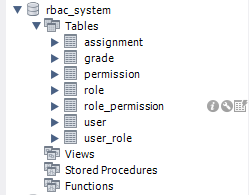
\includegraphics[width=\textwidth]{tables}
				\caption{Tables}
				\label{fig:tables}
			\end{figure}
			
			\newpage
			\item
			然后通过Hibernate的逆向工程生成相应的Entity类:
			\begin{figure}[H]
				\centering
				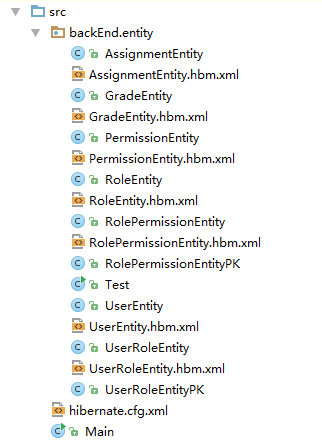
\includegraphics[width=\textwidth]{packages}
				\caption{Entities}
				\label{fig:packages}
			\end{figure}
			
			\newpage
			\item
			可是当我准备进行存取的时候,Hibernate报错了:
			\begin{figure}[H]
				\centering
				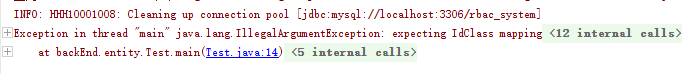
\includegraphics[width=\textwidth]{error}
				\caption{Error}
				\label{fig:error}
			\end{figure}
			
			\item
			到了最后也没有排查出来出错的原因,sign...
		\end{itemize}
	
		\item
		由于时间宝贵,我只能暂时放下这个已经快完成了后端的项目,而重新开始一个RBAC Demo。
		
		\item
		现在的想法是一个比上一个例子简单许多的Demo,想法如下:\\ 这个系统中包含了三种角色:管理员,教师和学生。管理员能查看所有的教师账户和学生账户,而教师只能查看所有的学生账户,学生不能查看别人的账户,此外,每种角色都有自己独有的按钮。系统在初始化的时候创建了一个管理员账户hello@hello.com并且系统以后也有且只有这一个管理员(因为注册选项没有注册为管理员的选项而只有教师和学生)。这次的技术选用在Android平台上。
		\begin{itemize}
			\item 先大概演示一下效果吧:
			\begin{enumerate}
				\item 这是app初始界面:可以注册成为老师或学生或登录。
				\begin{figure}[H]
					\centering
					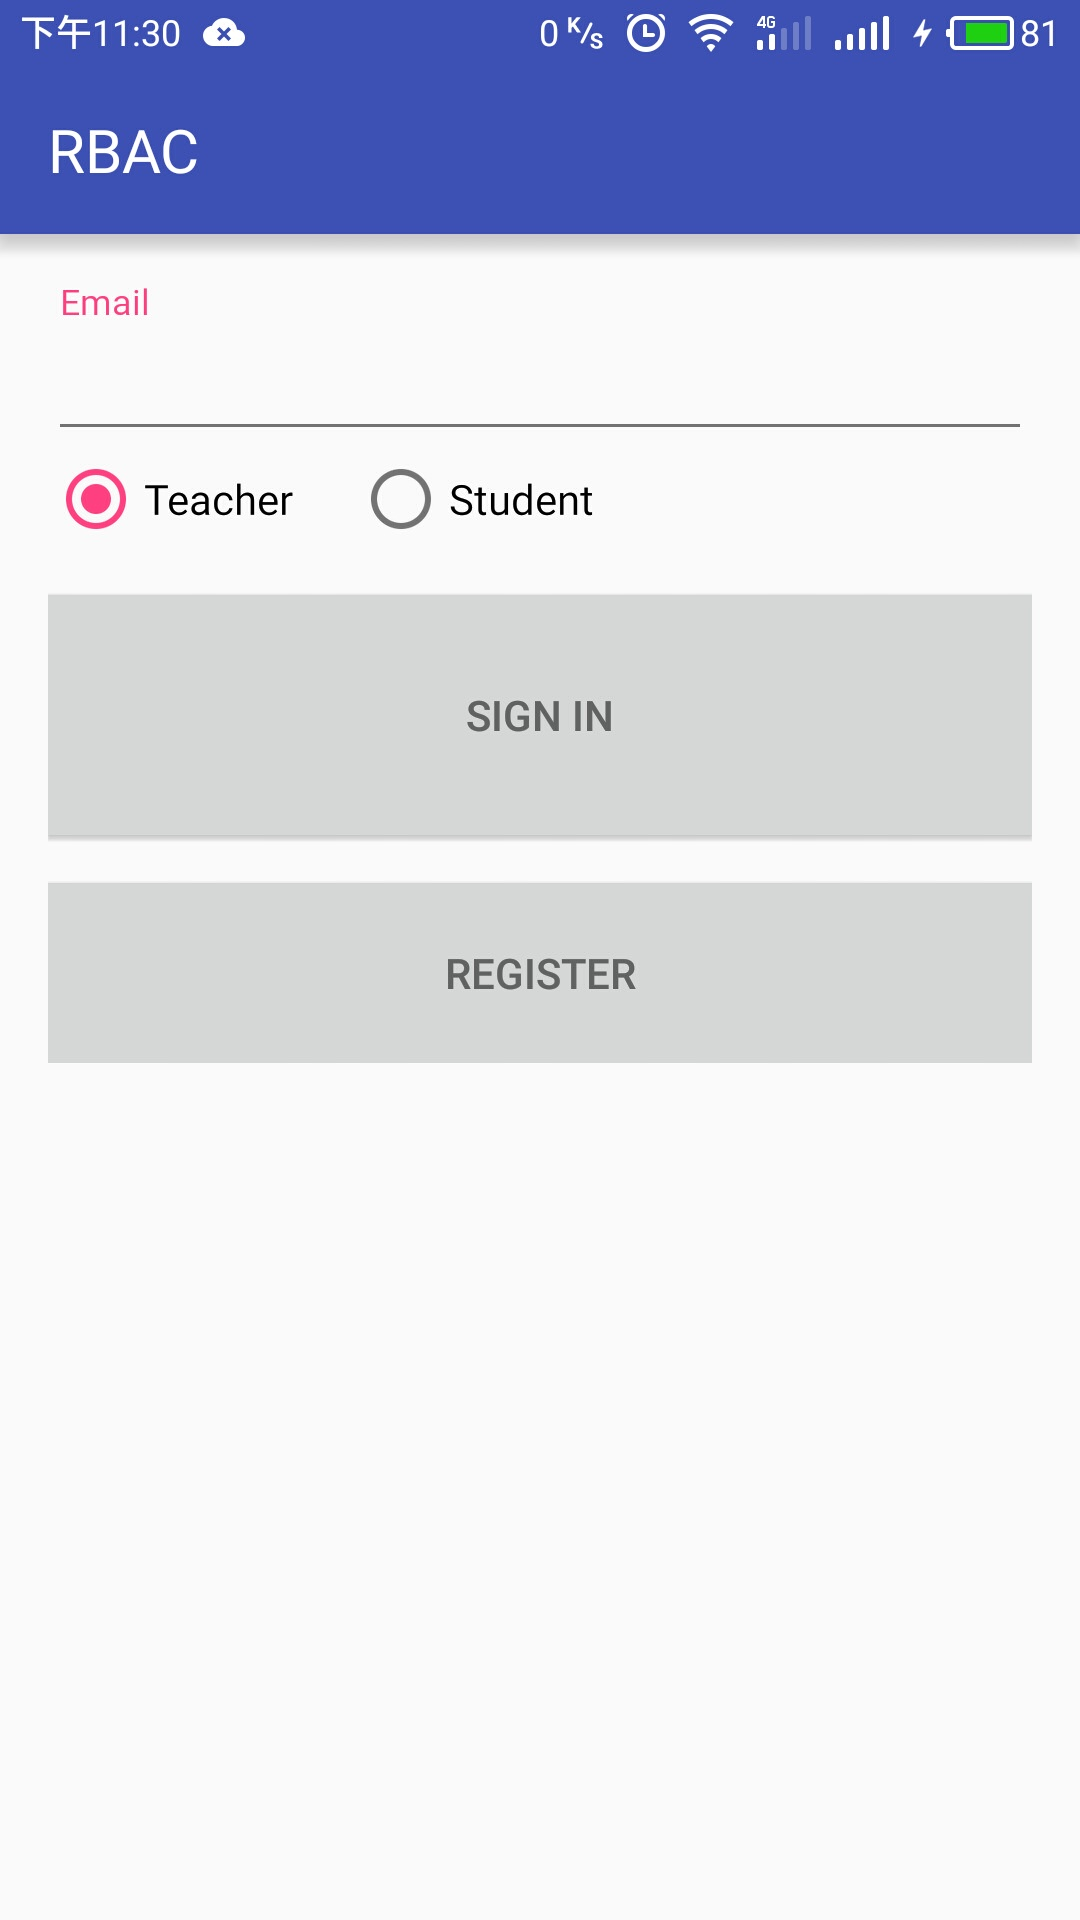
\includegraphics[height=0.3\textheight]{snapshot/1}
					\caption{初始界面}
					\label{fig:1}
				\end{figure}
				
				\item Email框有判断功能:
				\begin{figure}[H]
					\centering
					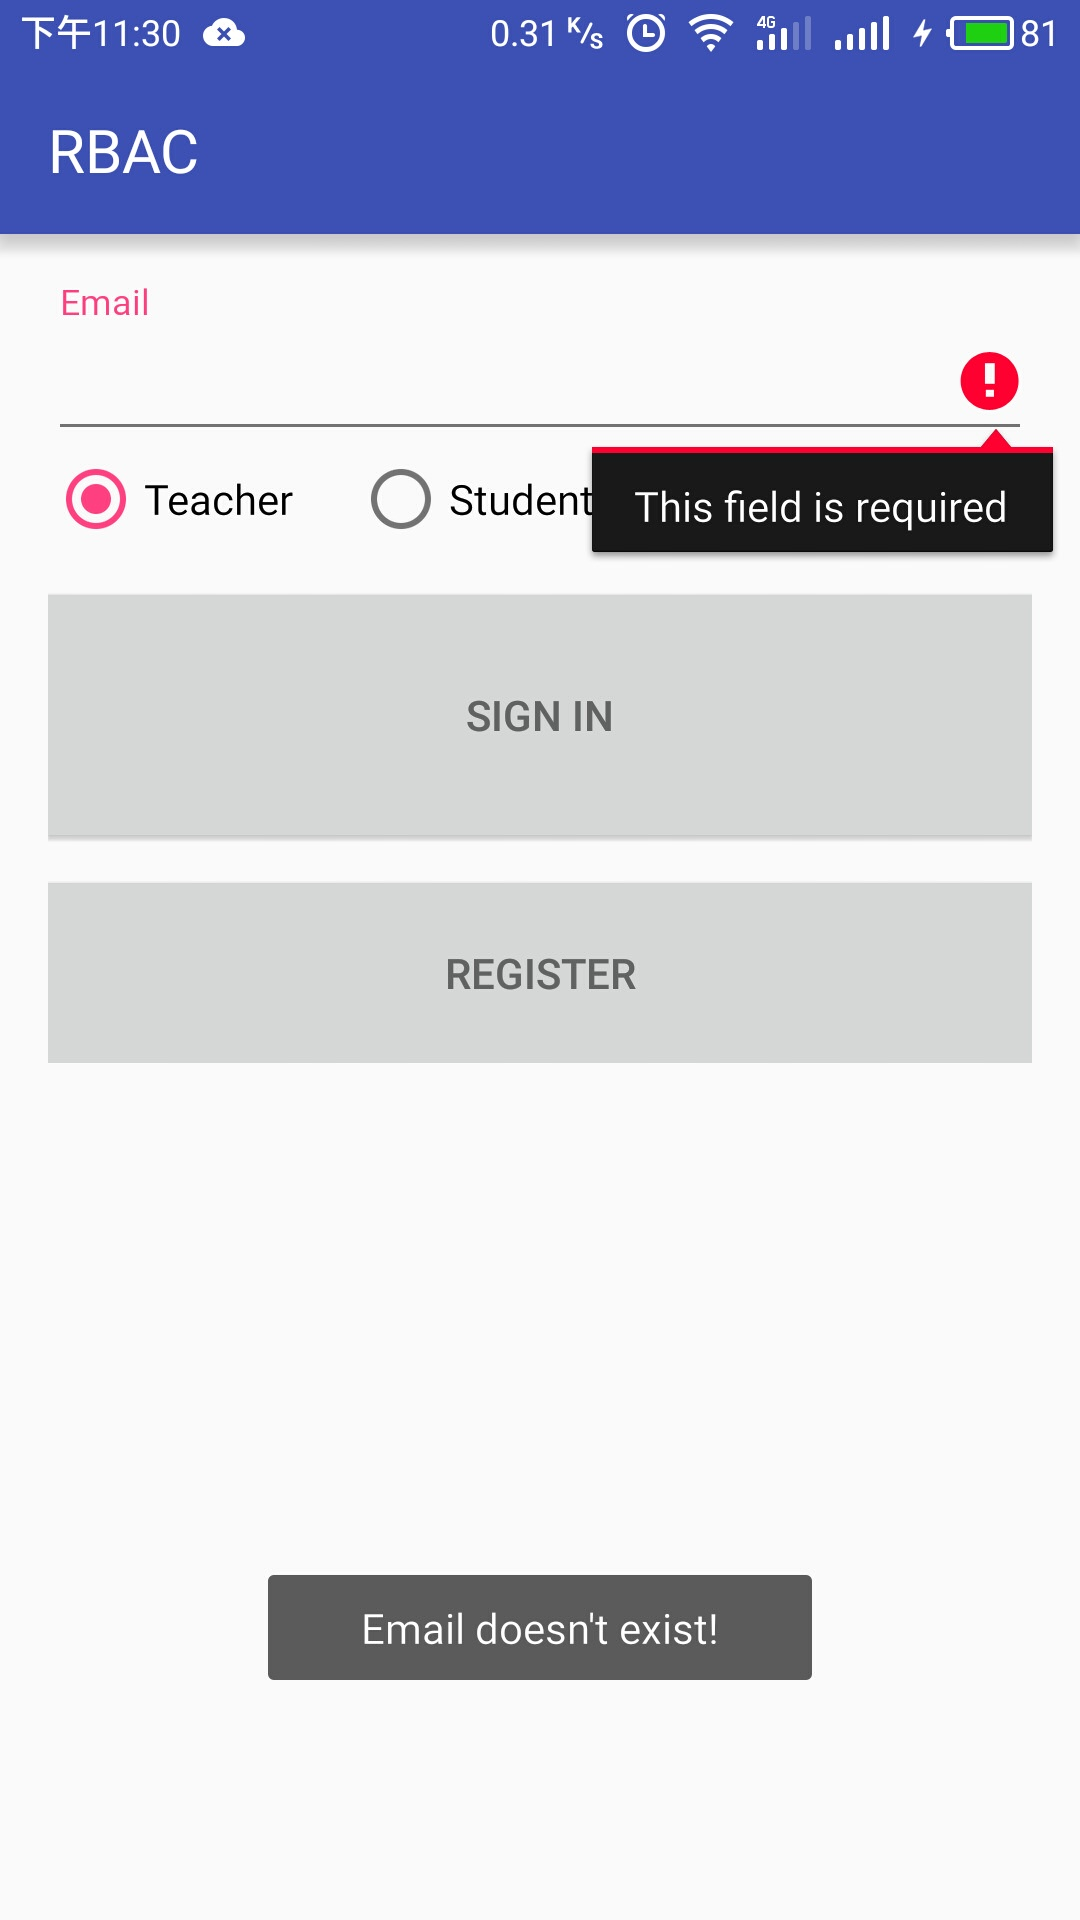
\includegraphics[height=0.39\textheight]{snapshot/2}
					\caption{Email判断}
					\label{fig:2}
				\end{figure}
				
				\item 先注册一个教师:
				\begin{figure}[H]
					\centering
					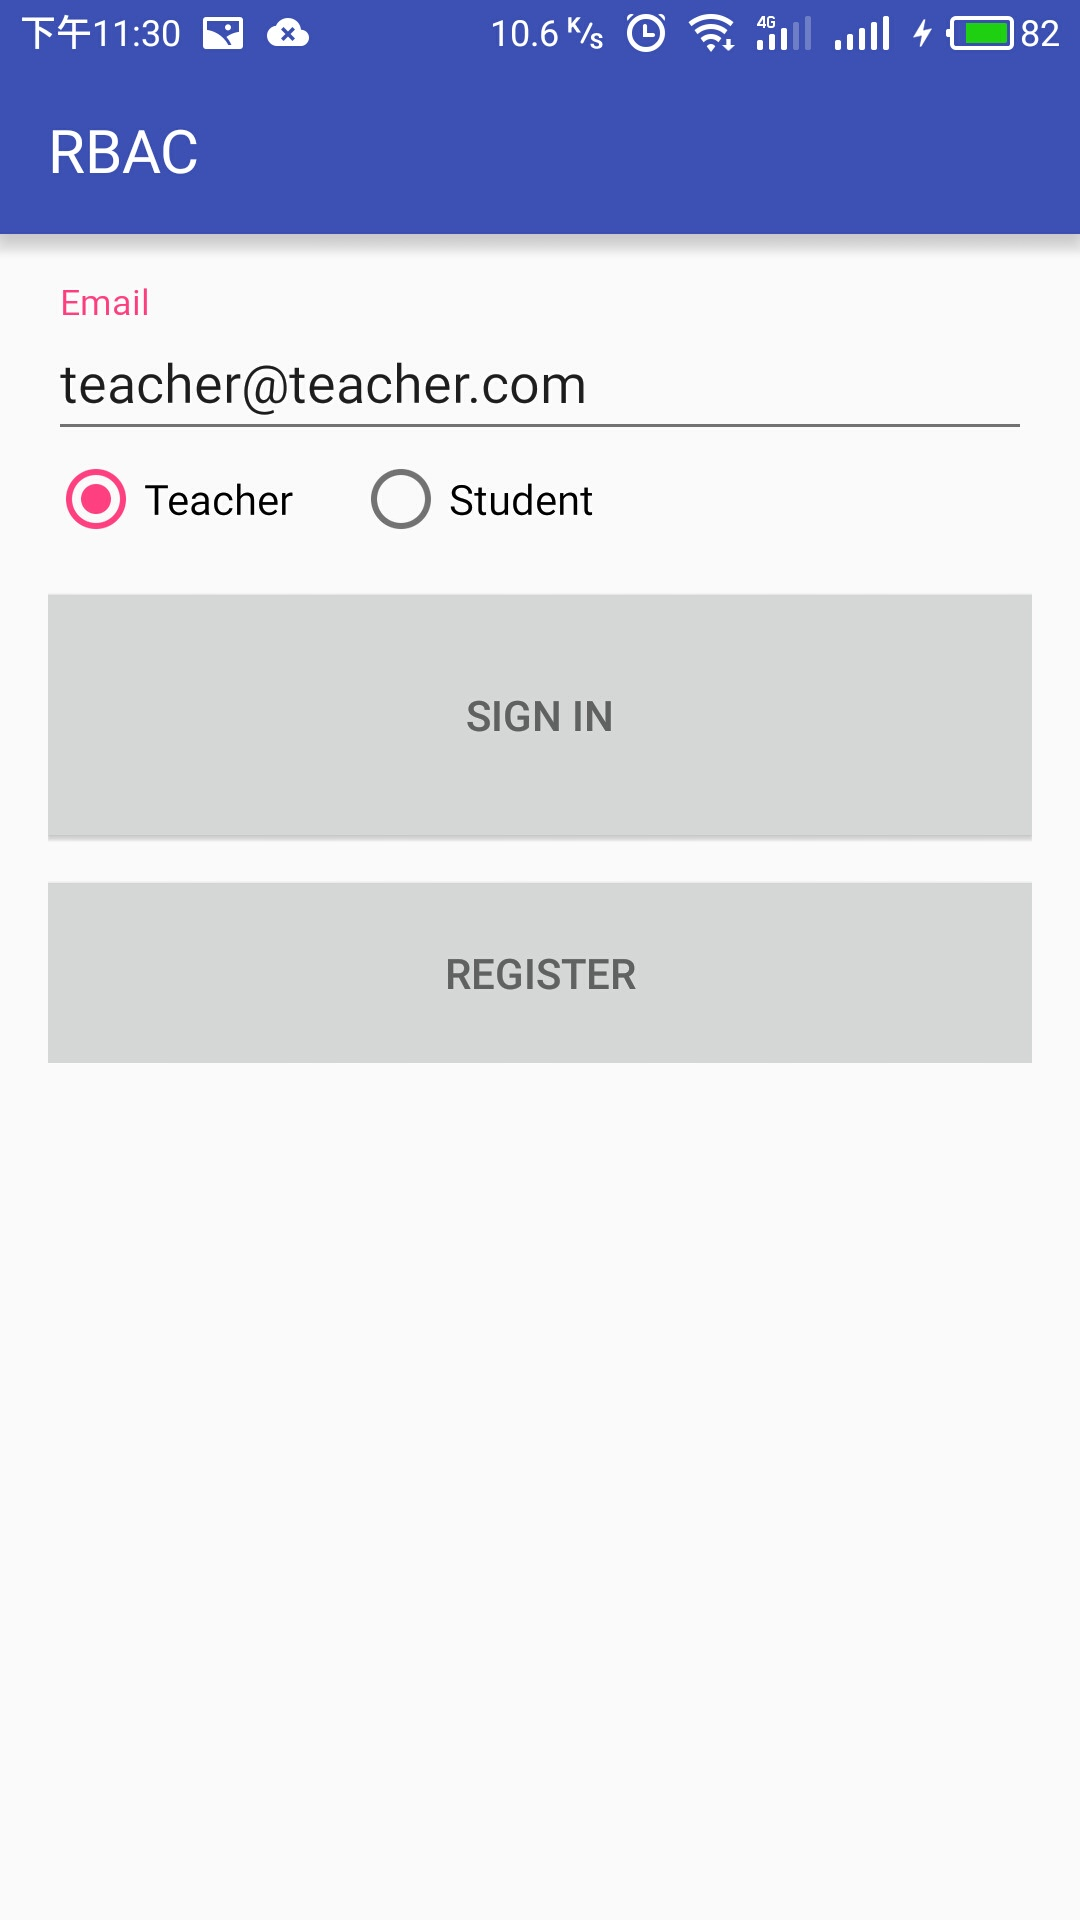
\includegraphics[height=0.39\textheight]{snapshot/3}
					\caption{教师注册}
					\label{fig:3}
				\end{figure}
				
				\item 若重复注册则会报提示信息:
				\begin{figure}[H]
					\centering
					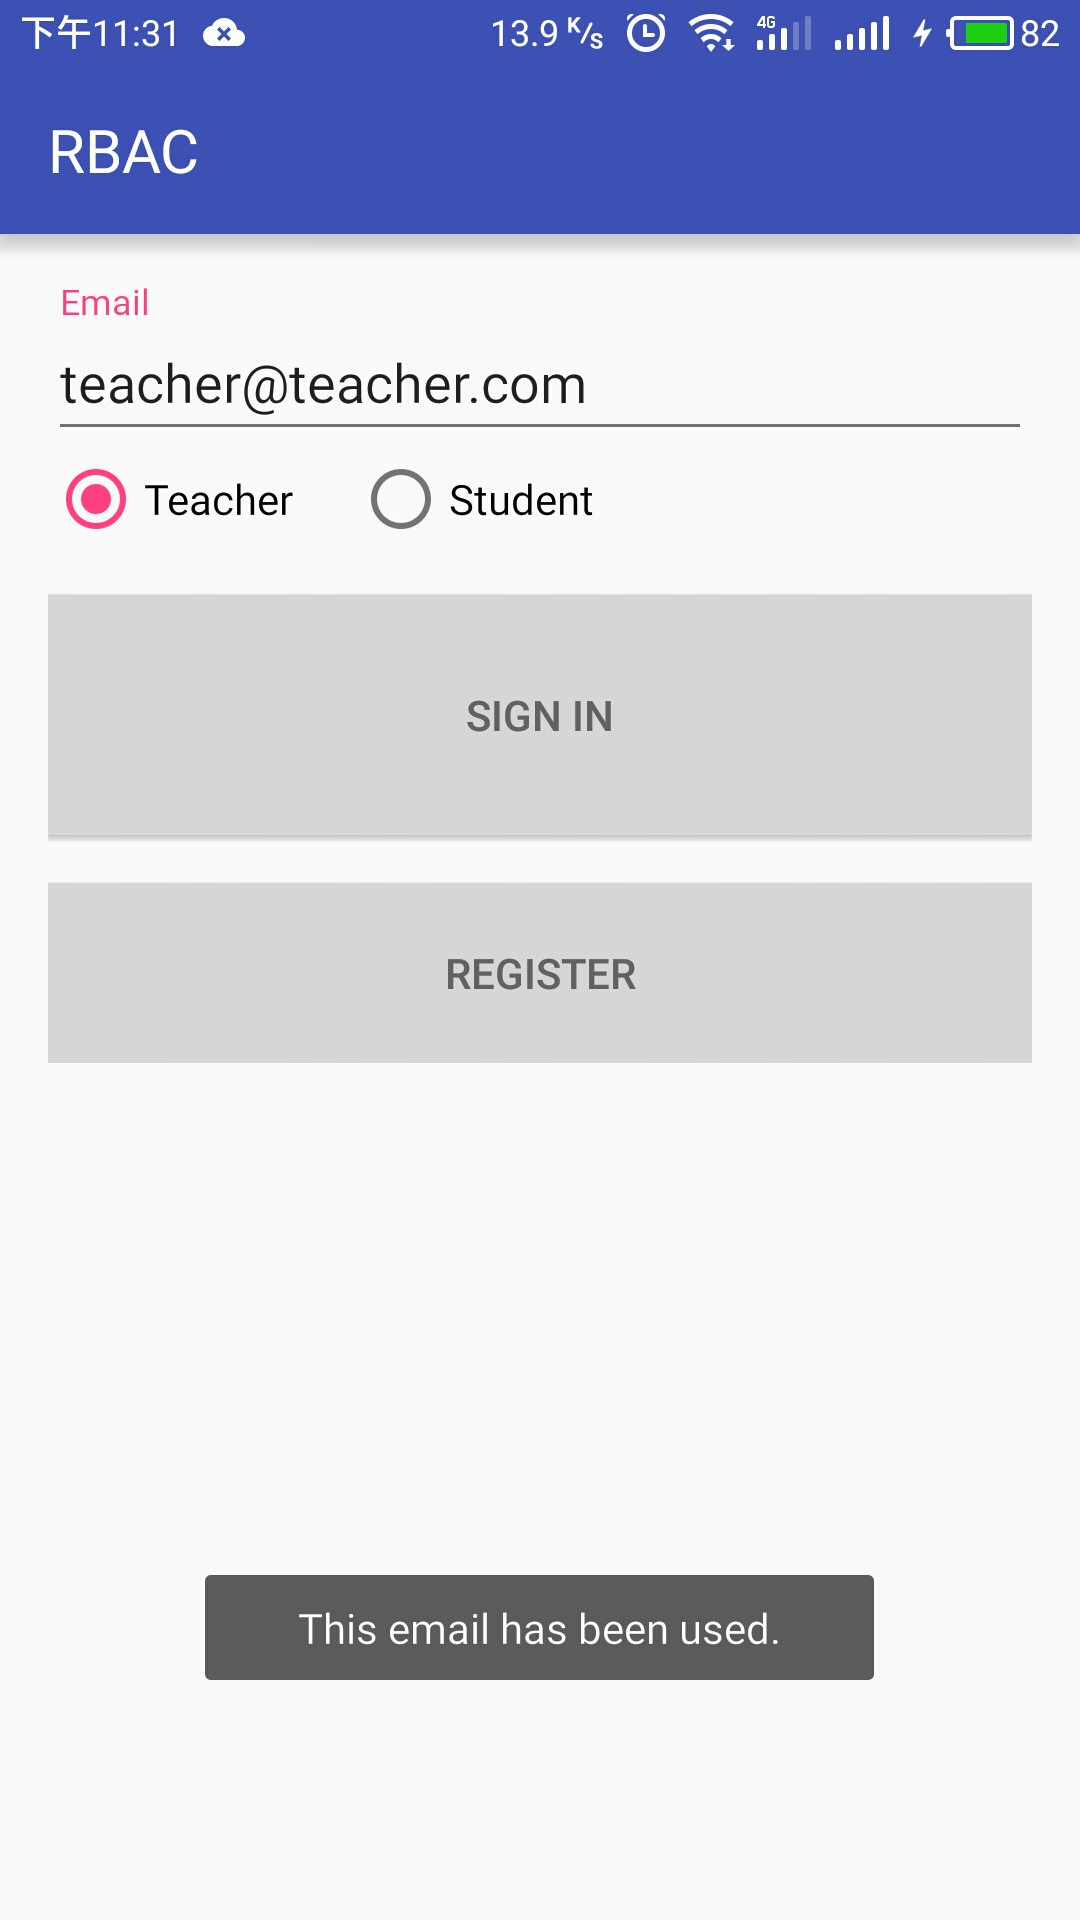
\includegraphics[height=0.39\textheight]{snapshot/4}
					\caption{Email重复}
					\label{fig:4}
				\end{figure}
				
				\item 教师登入界面如下:
				\begin{figure}[H]
					\centering
					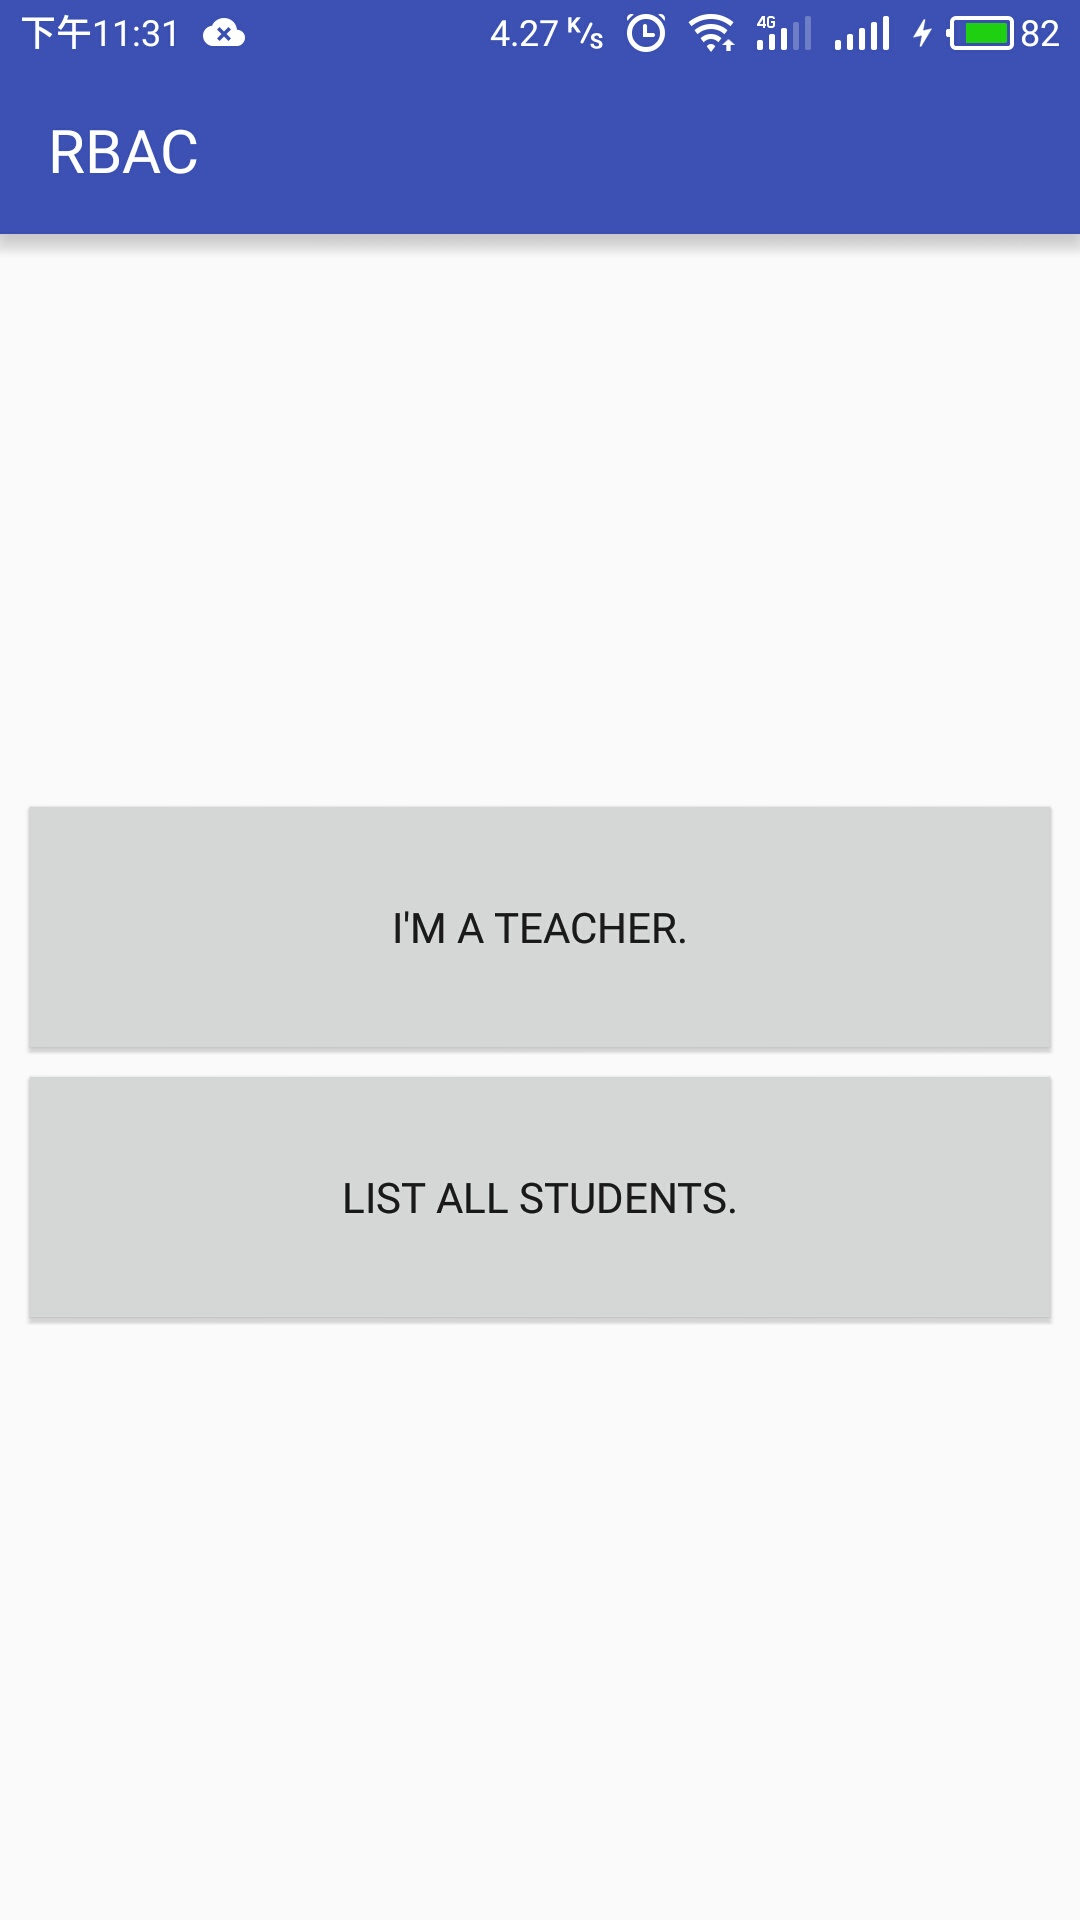
\includegraphics[height=0.39\textheight]{snapshot/5}
					\caption{教师登入界面}
					\label{fig:5}
				\end{figure}
			
				\item 单击第一个Button:
				\begin{figure}[H]
					\centering
					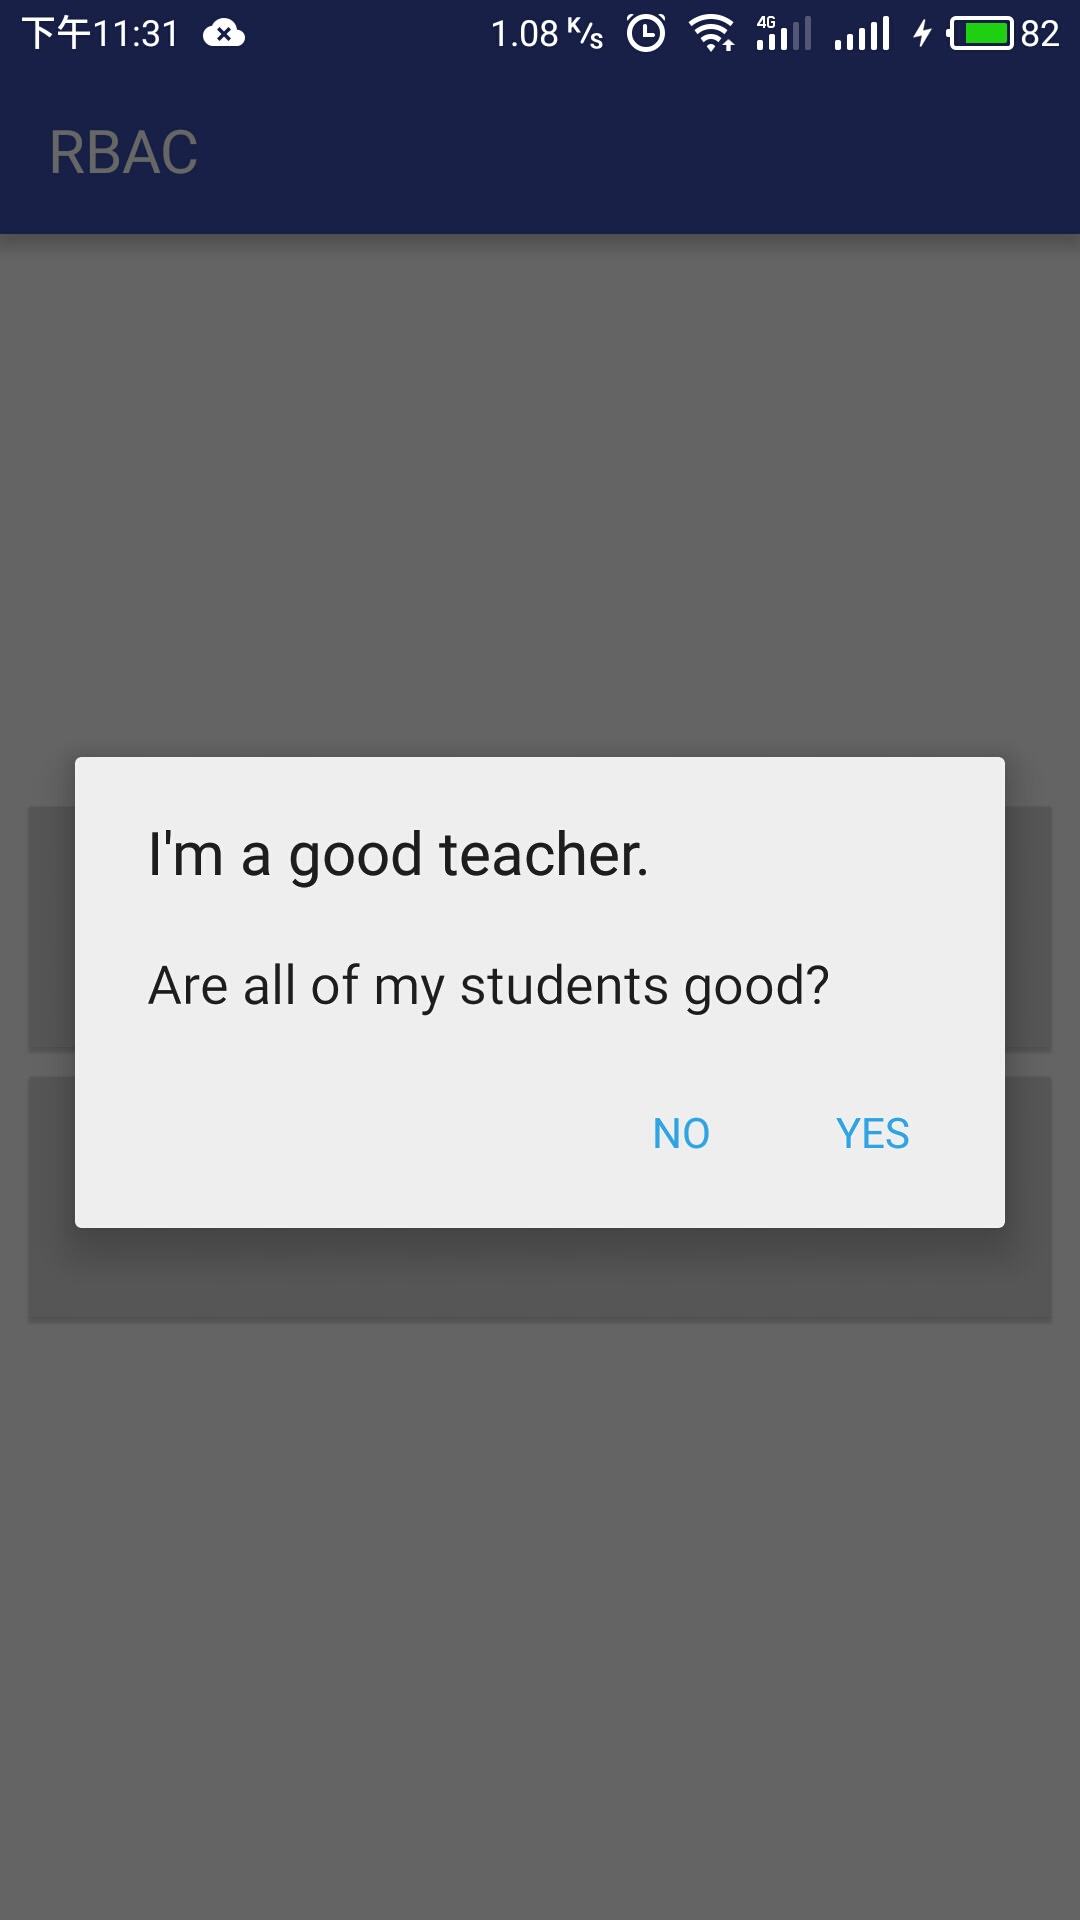
\includegraphics[height=0.39\textheight]{snapshot/6}
					\caption{按钮点击}
					\label{fig:6}
				\end{figure}
				
				\item 单击Yes:
				\begin{figure}[H]
					\centering
					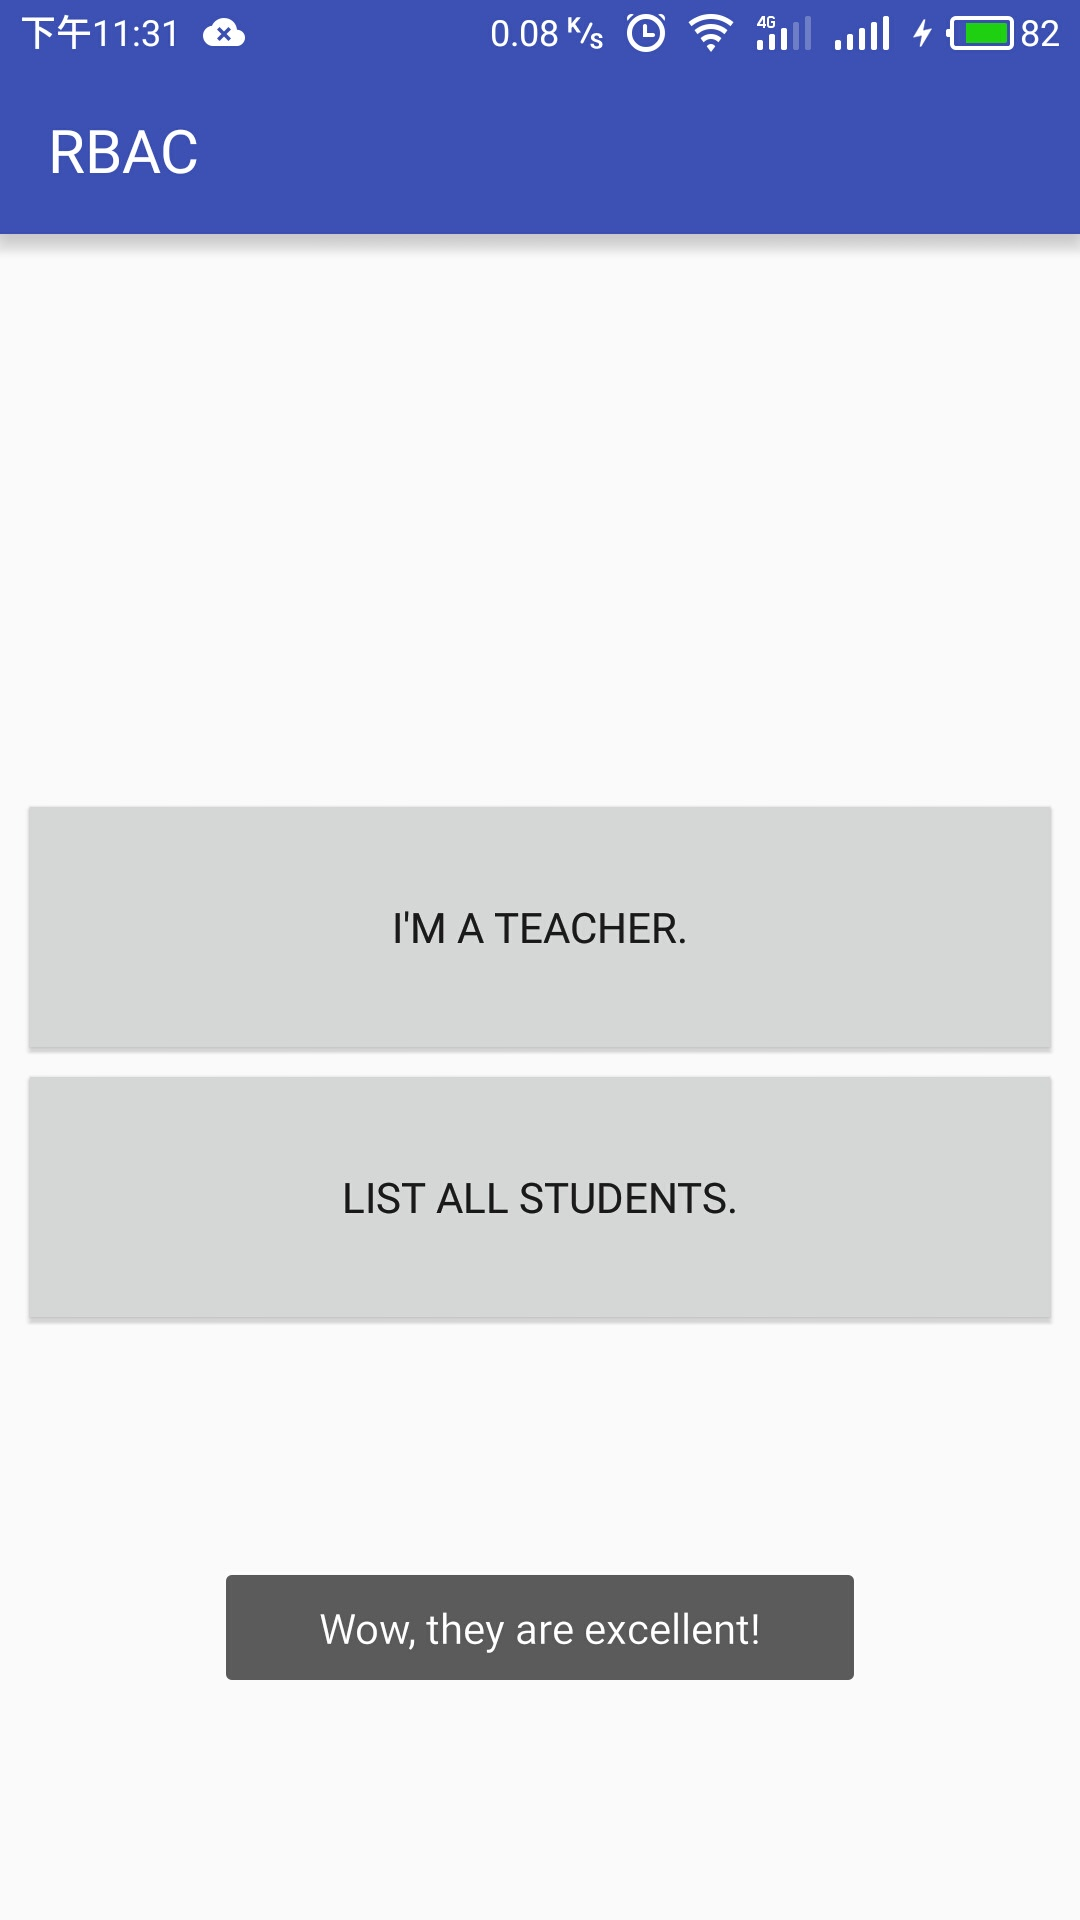
\includegraphics[height=0.39\textheight]{snapshot/7}
					\caption{按钮点击}
					\label{fig:7}
				\end{figure}
			
				\item 注册一个学生:
				\begin{figure}[H]
					\centering
					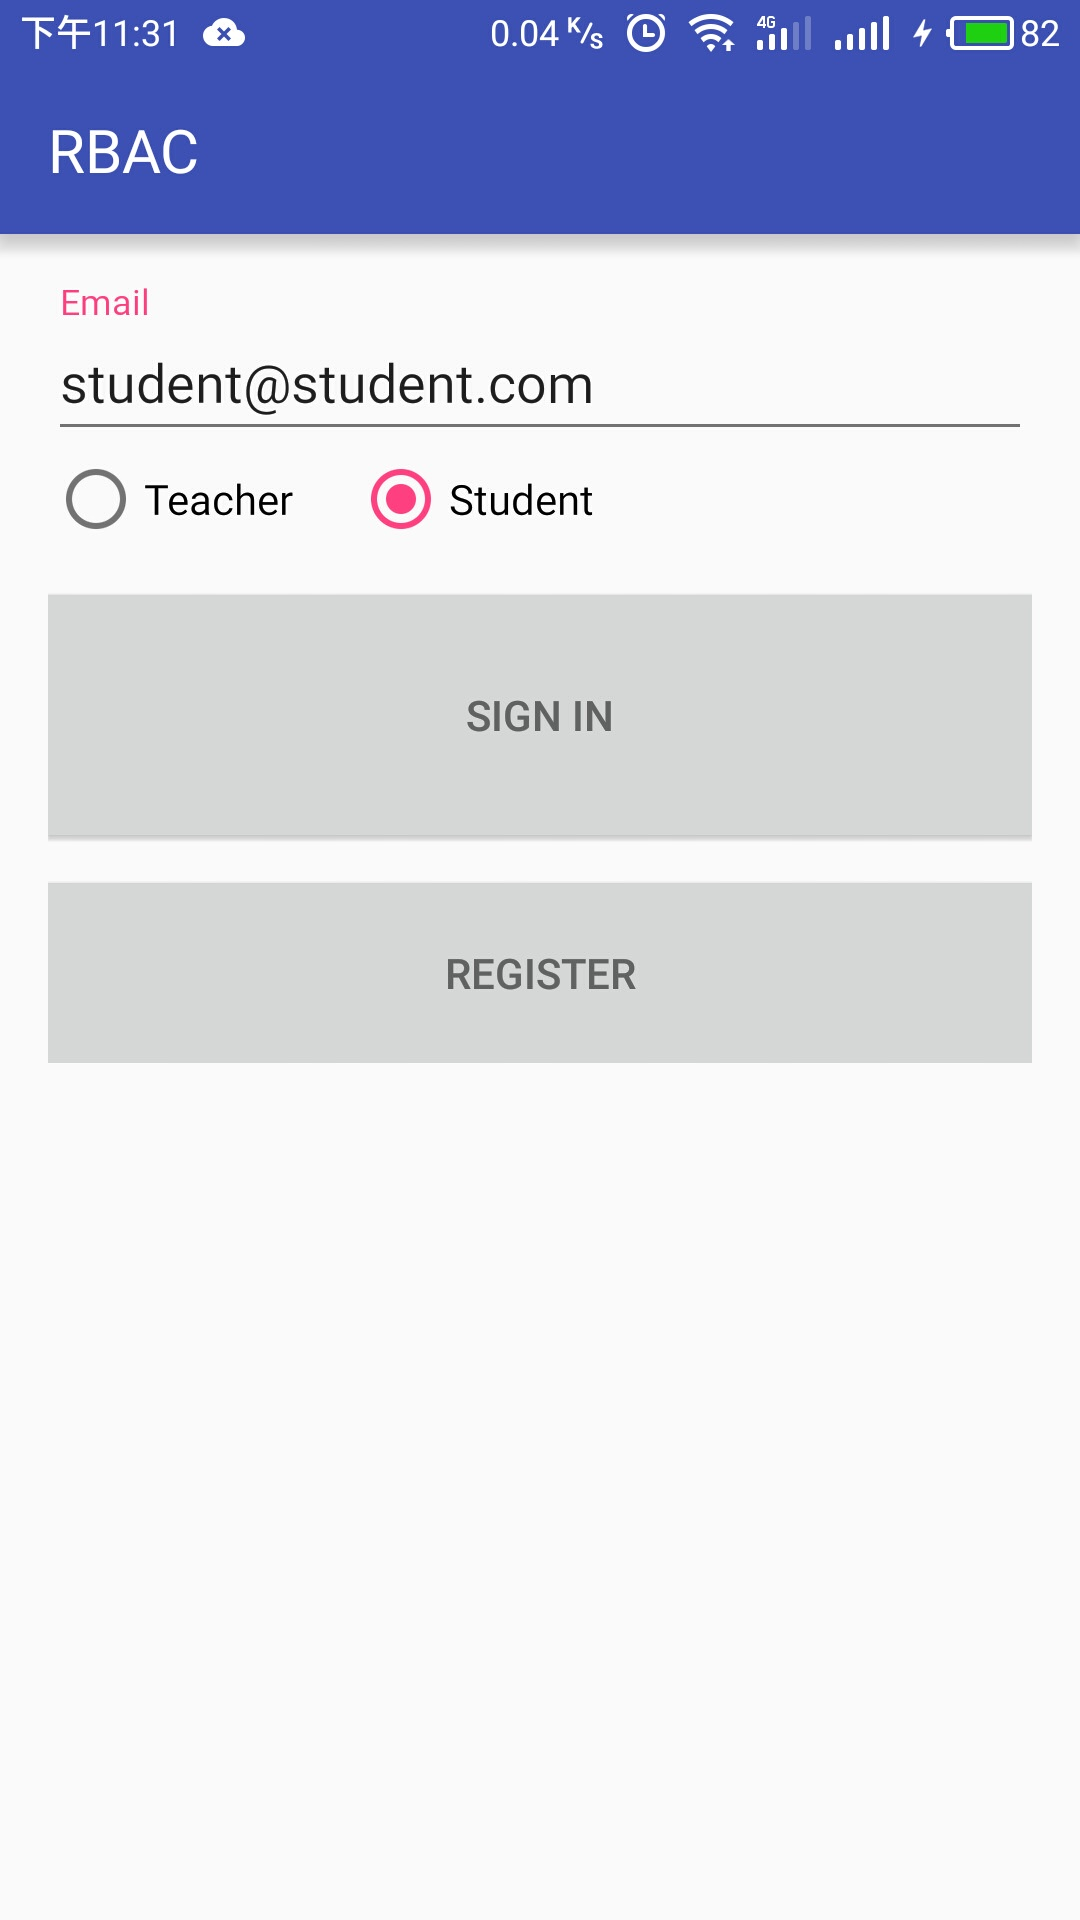
\includegraphics[height=0.39\textheight]{snapshot/8}
					\caption{注册学生}
					\label{fig:8}
				\end{figure}
			
				\item 学生只有一个Button:
				\begin{figure}[H]
					\centering
					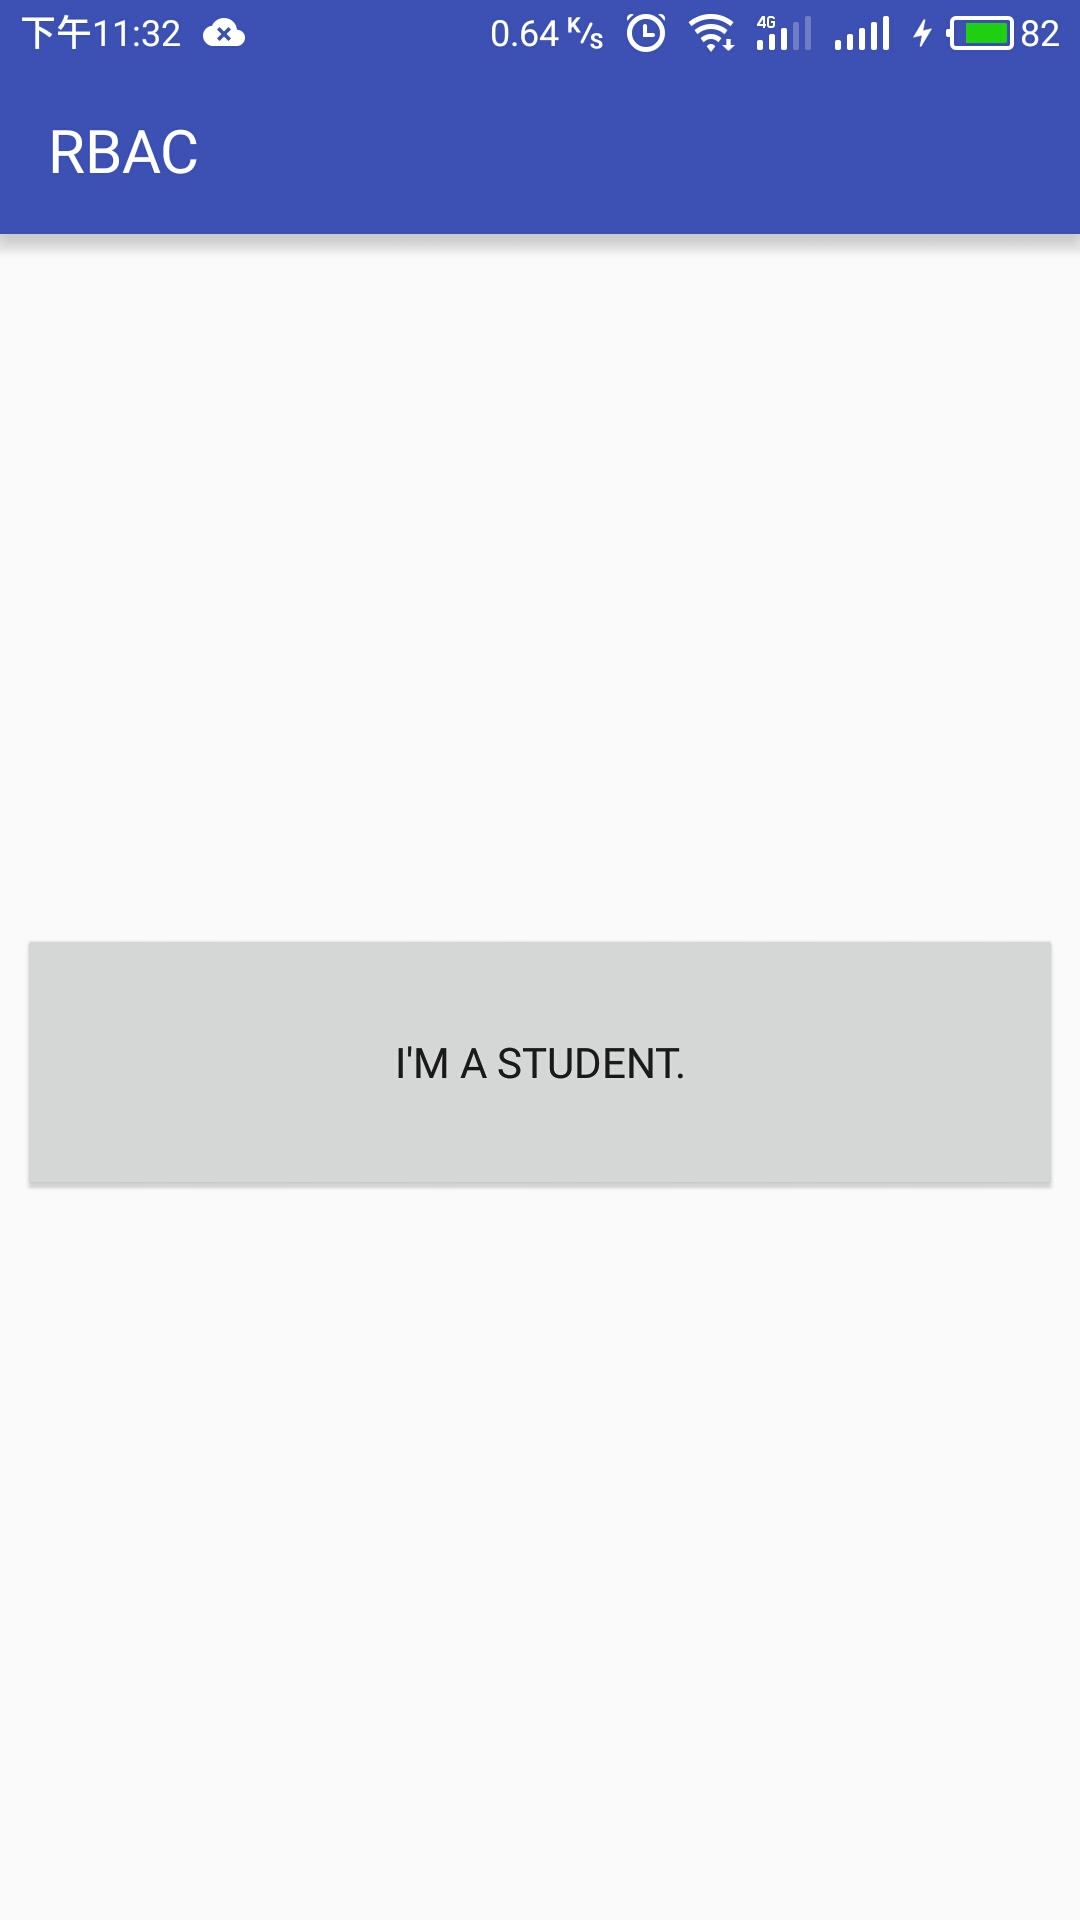
\includegraphics[height=0.39\textheight]{snapshot/9}
					\caption{学生登入界面}
					\label{fig:9}
				\end{figure}
			
				\item 单击Button:
				\begin{figure}[H]
					\centering
					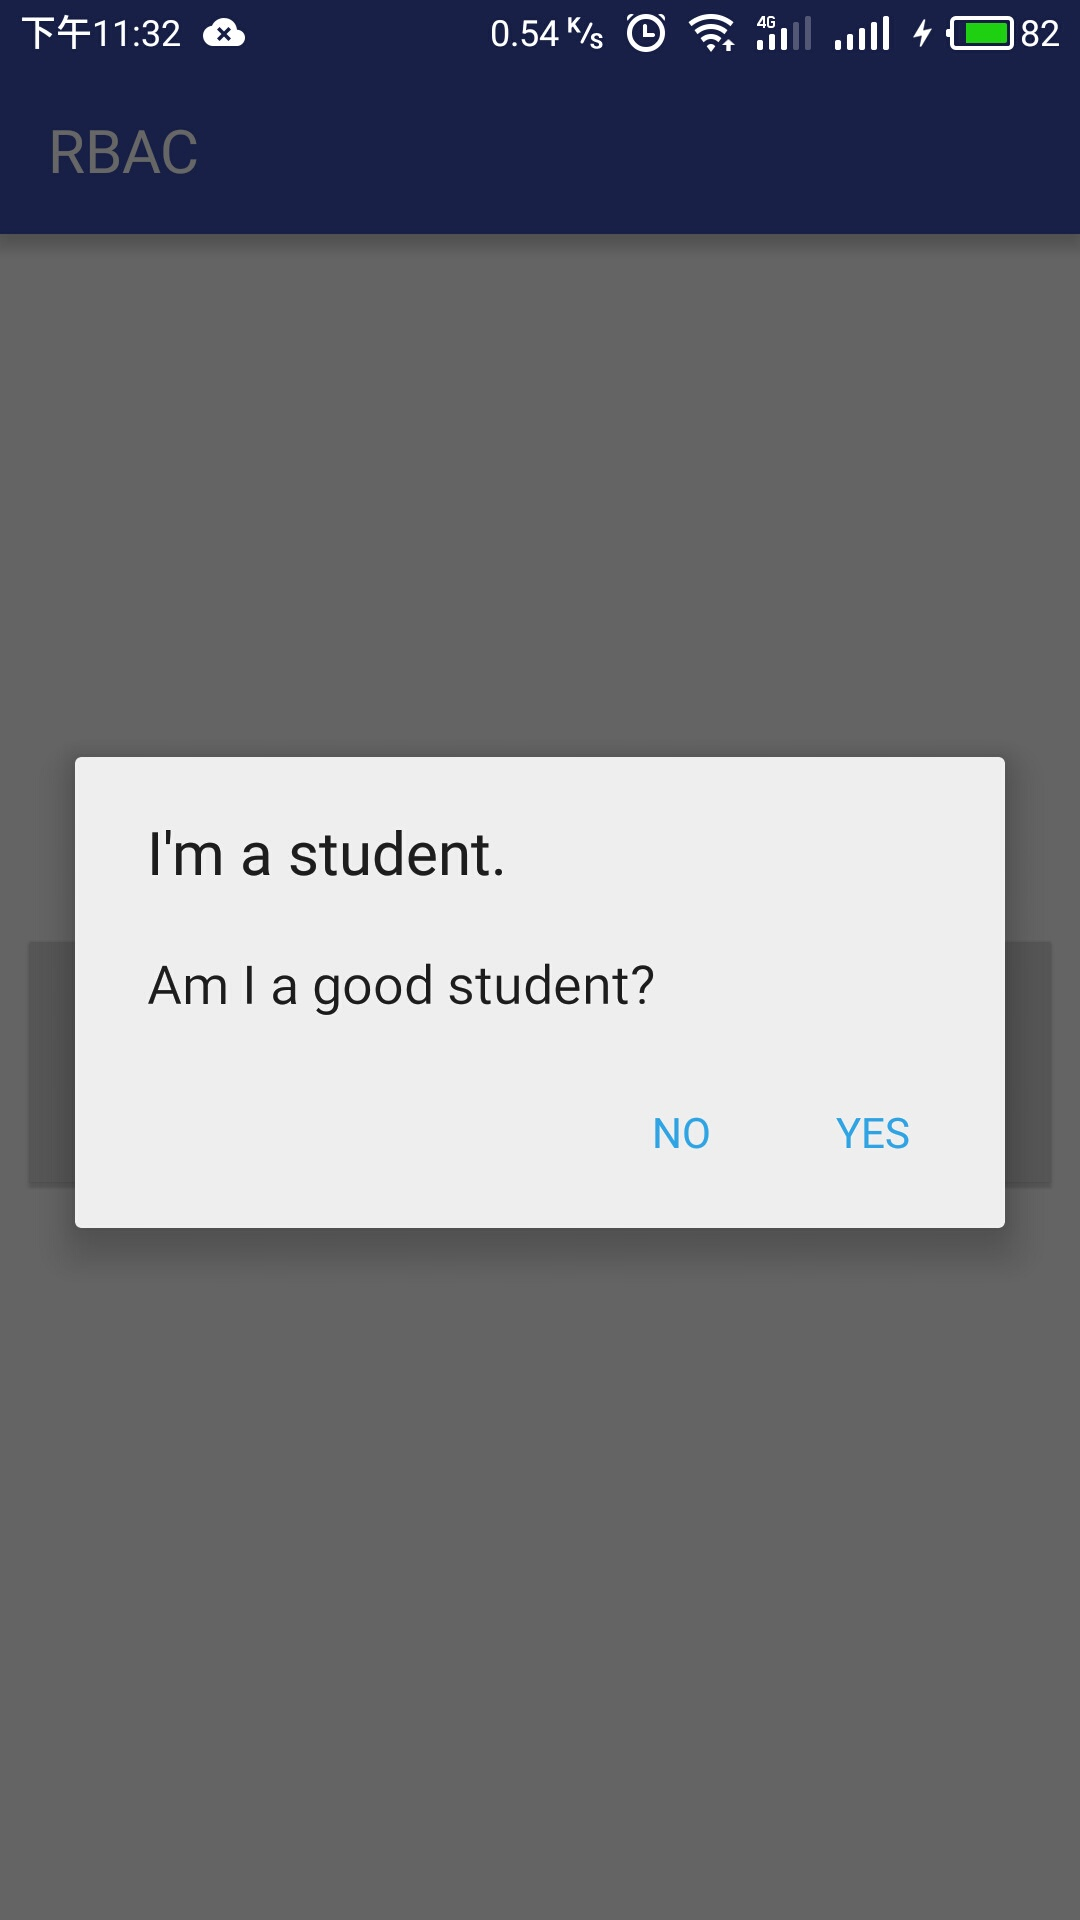
\includegraphics[height=0.39\textheight]{snapshot/10}
					\caption{按钮点击}
					\label{fig:10}
				\end{figure}
			
				\item 单击Yes:
				\begin{figure}[H]
					\centering
					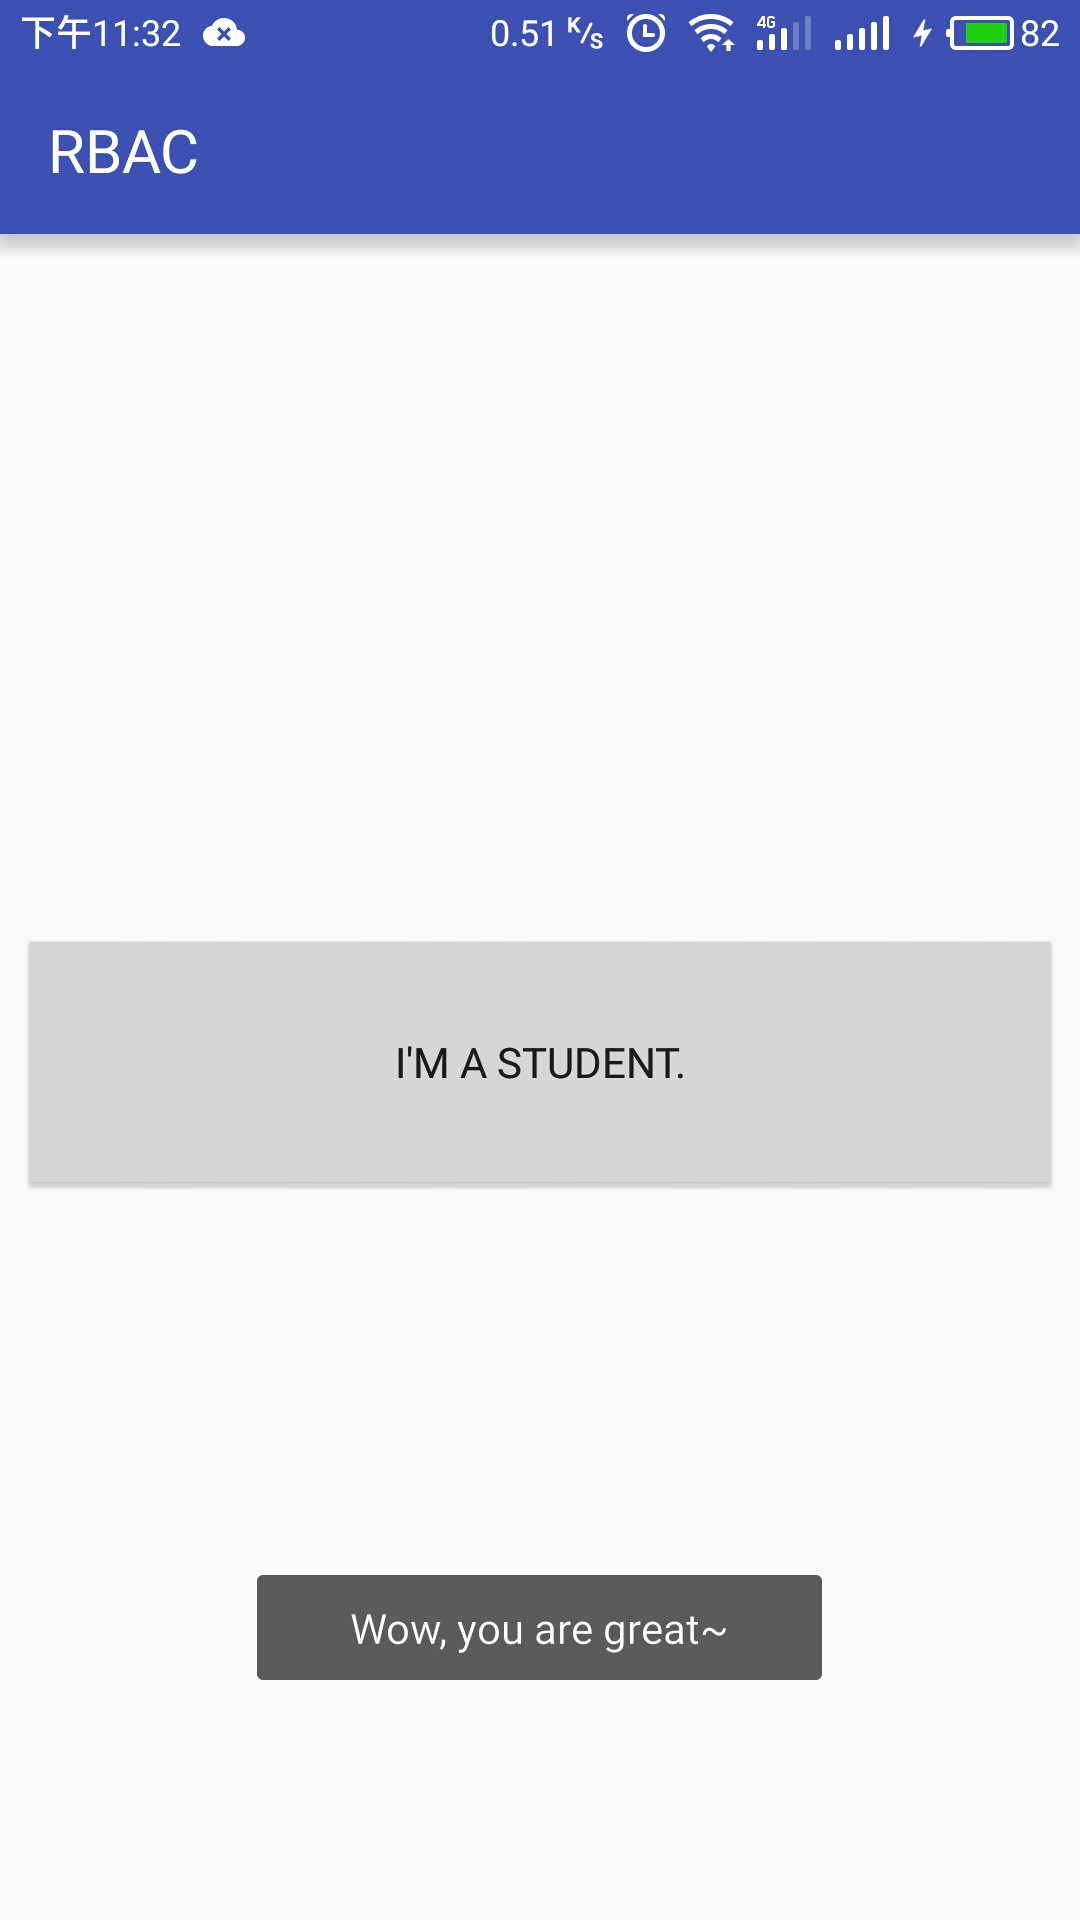
\includegraphics[height=0.39\textheight]{snapshot/11}
					\caption{按钮点击}
					\label{fig:11}
				\end{figure}
			
				\item 再次登入教师账号点击第二个按钮,可以查看到刚刚注册的学生:
				\begin{figure}[H]
					\centering
					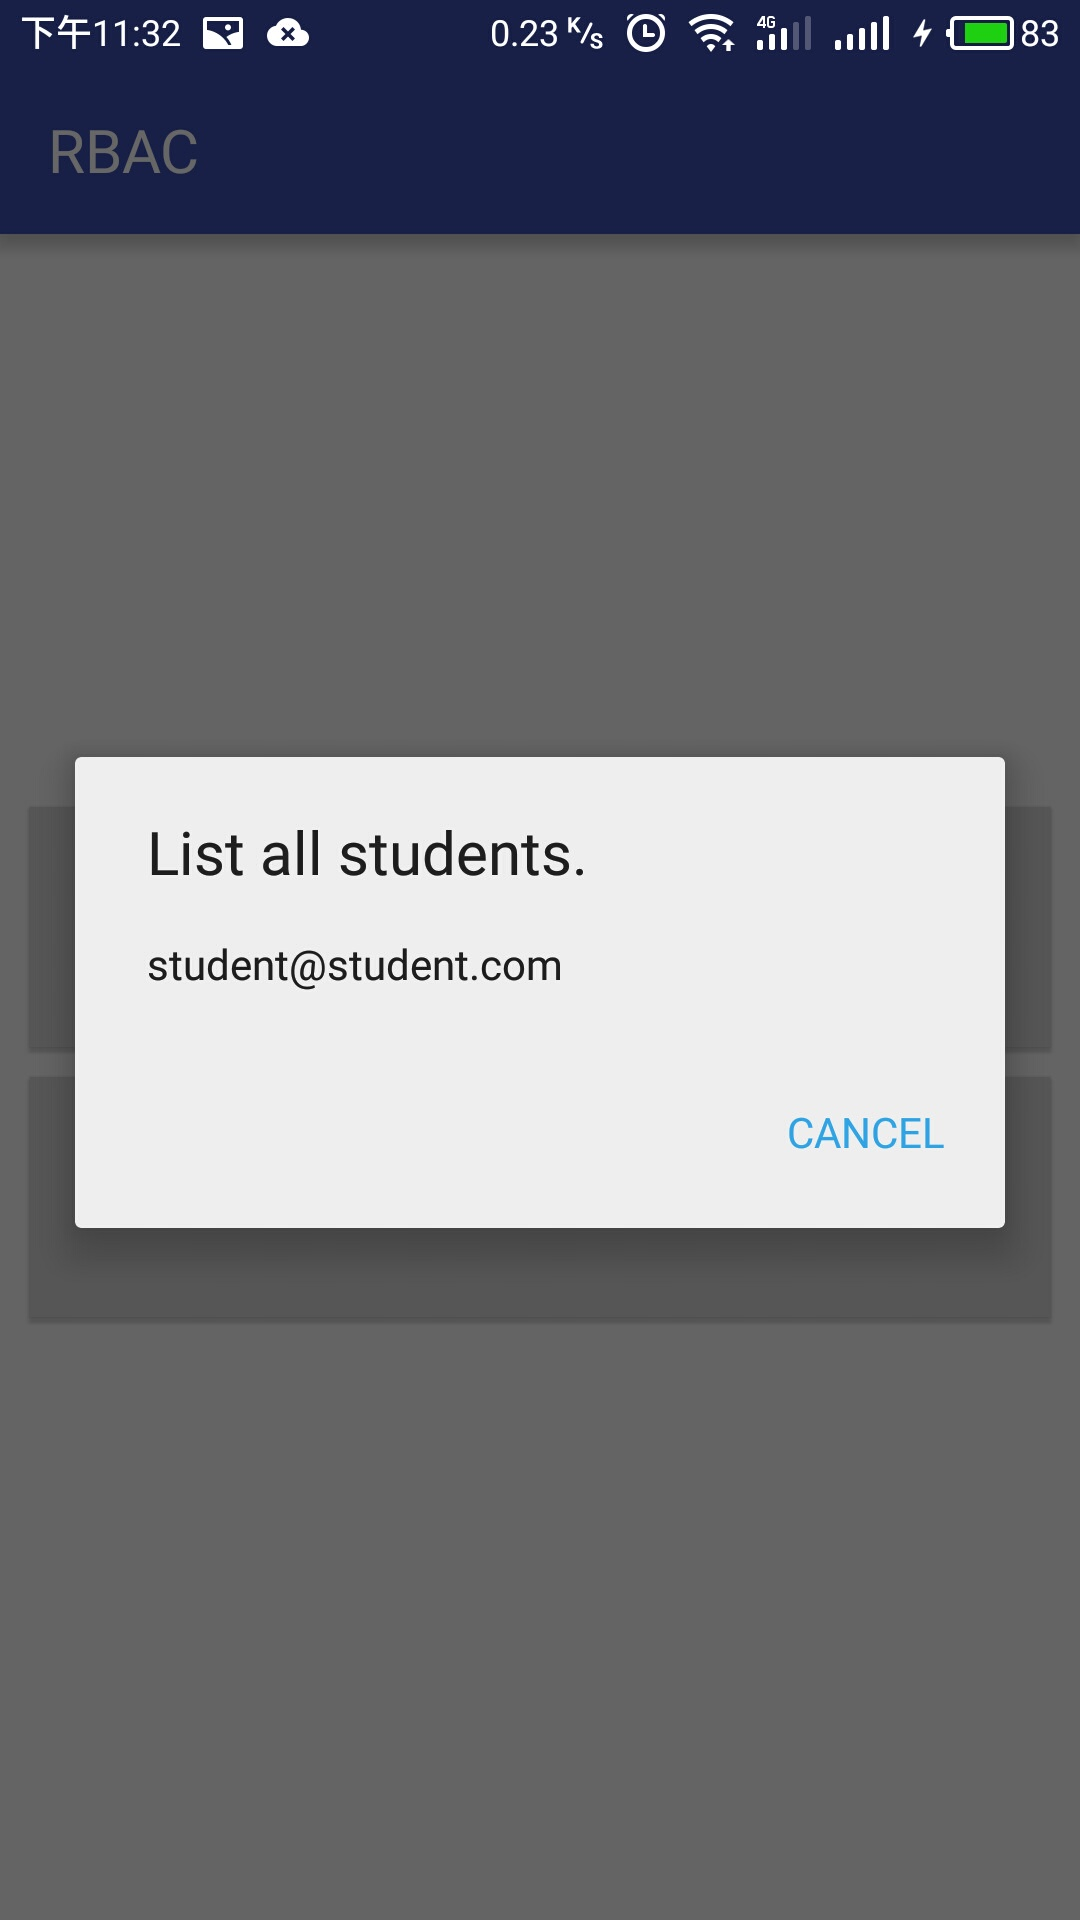
\includegraphics[height=0.35\textheight]{snapshot/12}
					\caption{教师查看学生}
					\label{fig:12}
				\end{figure}
			
				\item 系统中固有一个管理员,所以不可注册重名账户:
				\begin{figure}[H]
					\centering
					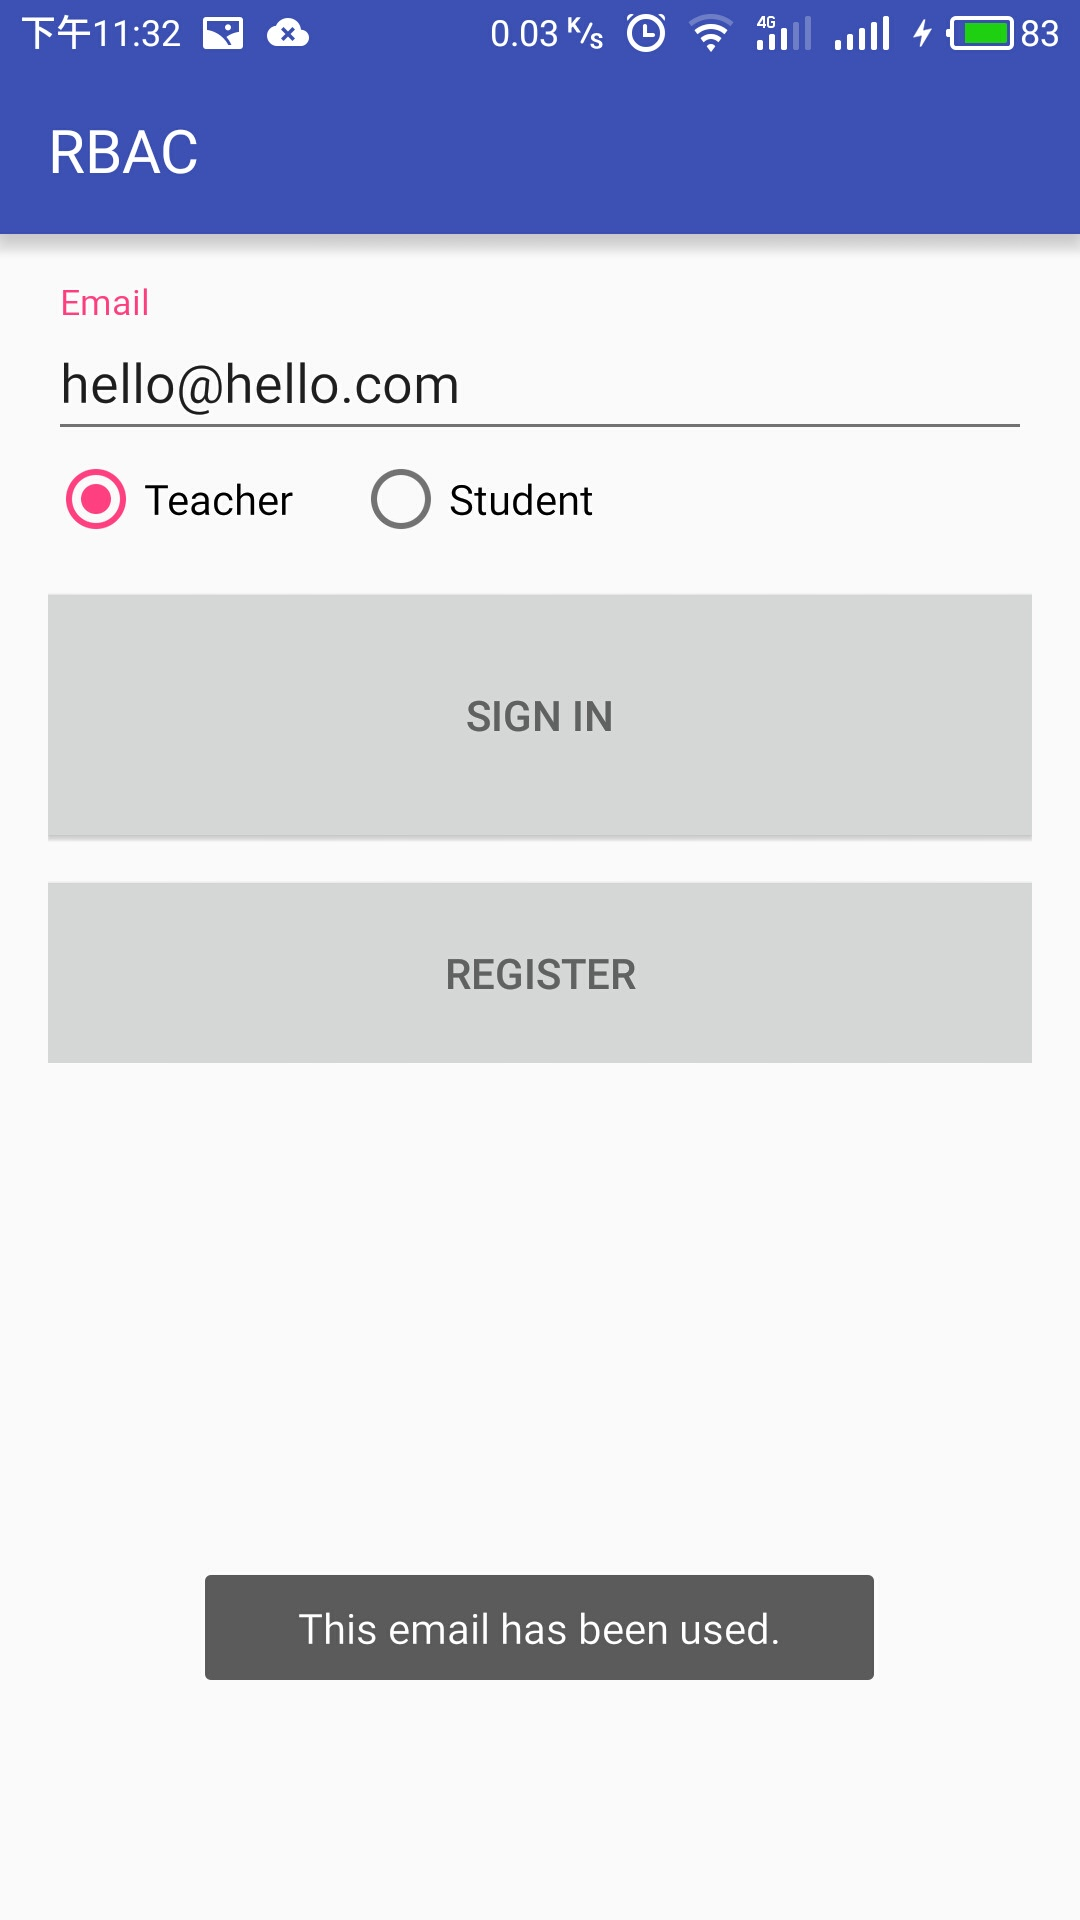
\includegraphics[height=0.39\textheight]{snapshot/13}
					\caption{尝试注册管理员账号}
					\label{fig:13}
				\end{figure}
			
				\item 管理员登入界面:
				\begin{figure}[H]
					\centering
					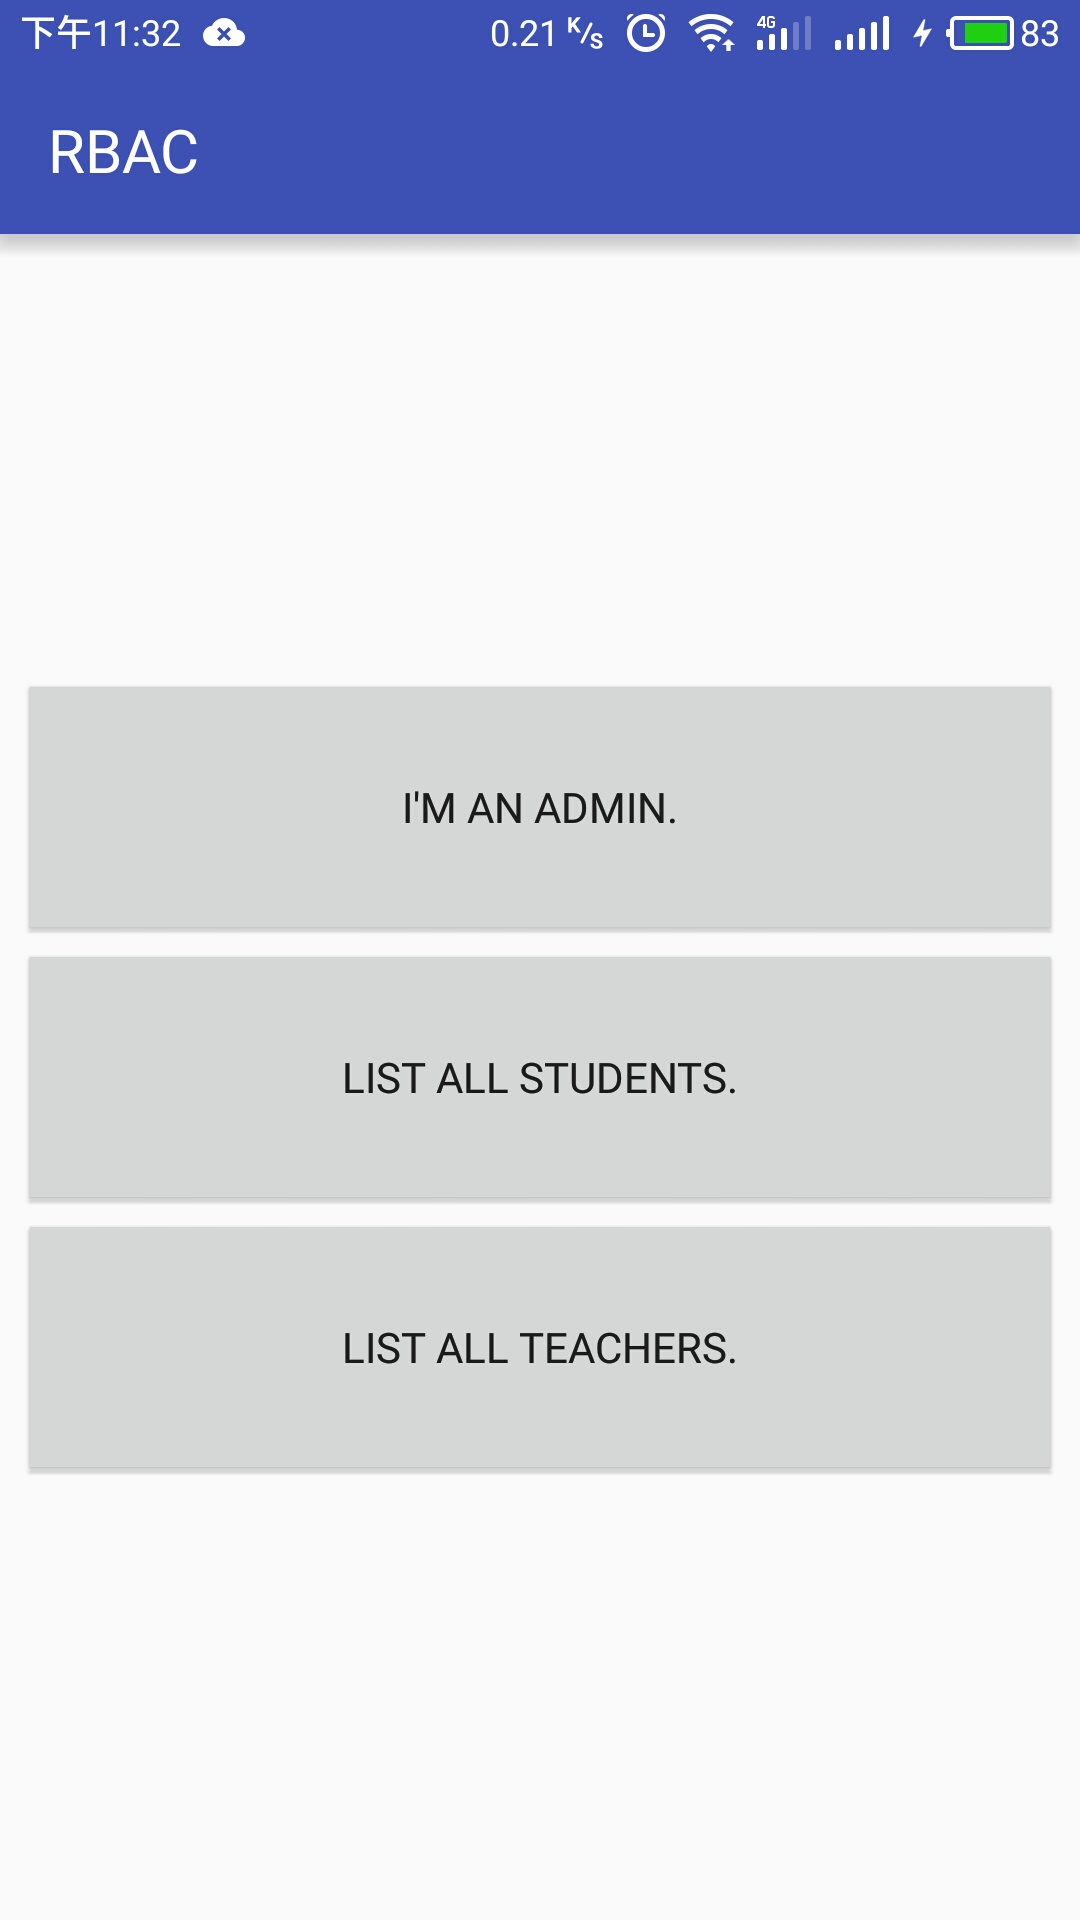
\includegraphics[height=0.39\textheight]{snapshot/14}
					\caption{管理员登入}
					\label{fig:14}
				\end{figure}
			
				\item 单击第一个Button:
				\begin{figure}[H]
					\centering
					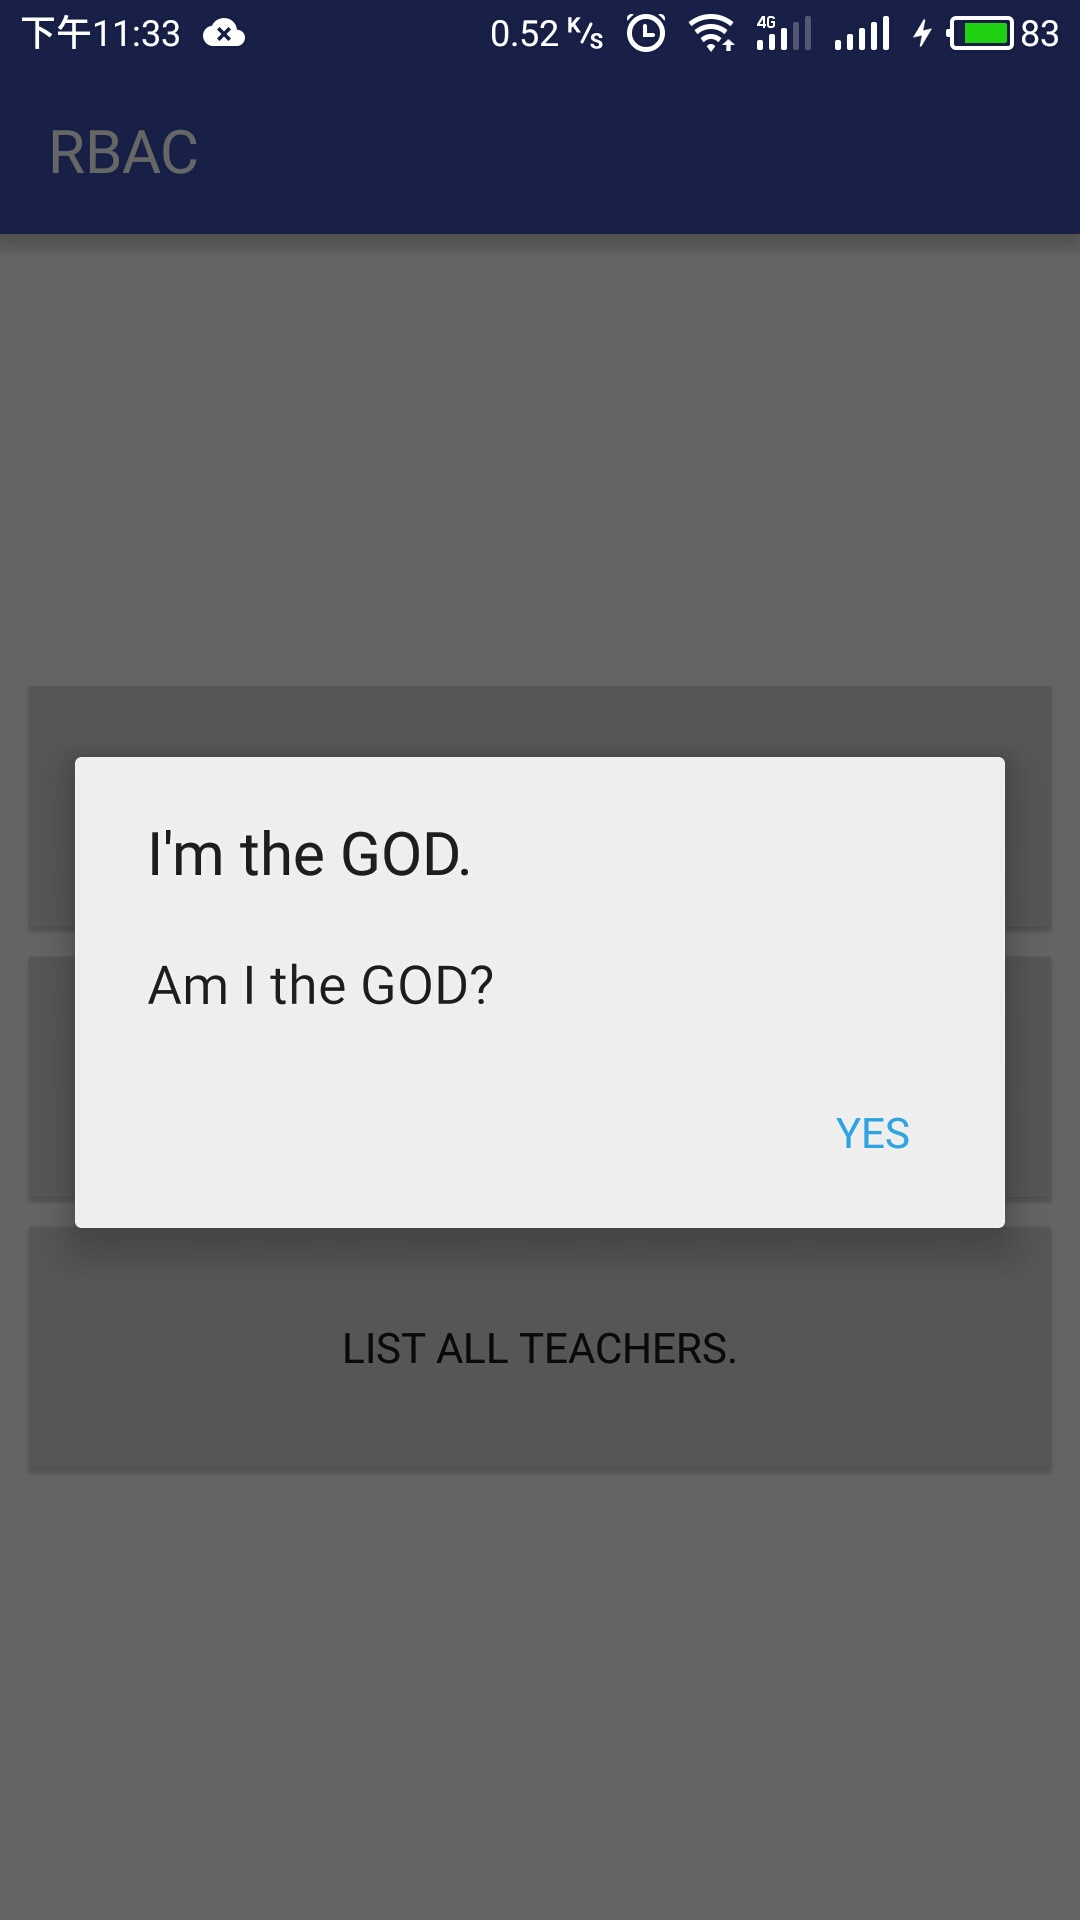
\includegraphics[height=0.39\textheight]{snapshot/15}
					\caption{按钮点击}
					\label{fig:15}
				\end{figure}
			
				\item 单击Yes:
				\begin{figure}[H]
					\centering
					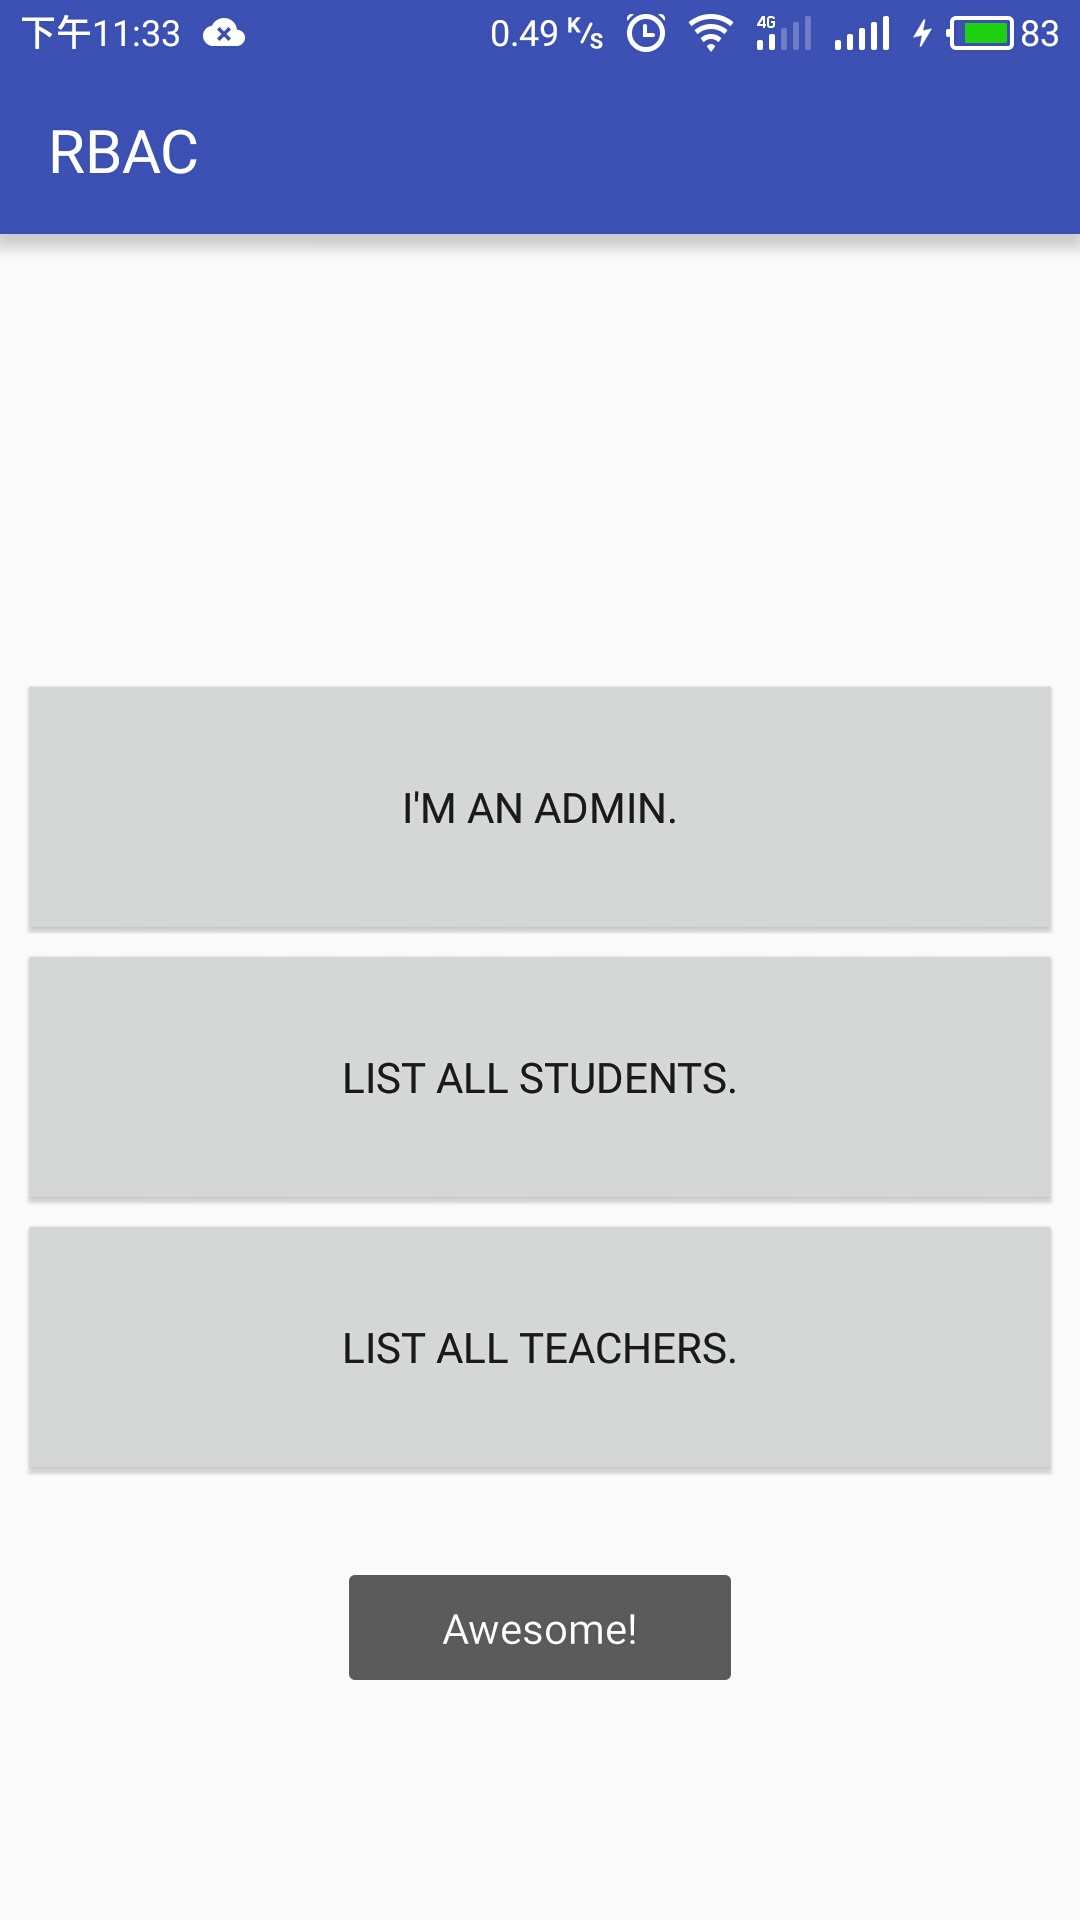
\includegraphics[height=0.39\textheight]{snapshot/16}
					\caption{按钮点击}
					\label{fig:16}
				\end{figure}
			
				\item 管理员查看学生用户:
				\begin{figure}[H]
					\centering
					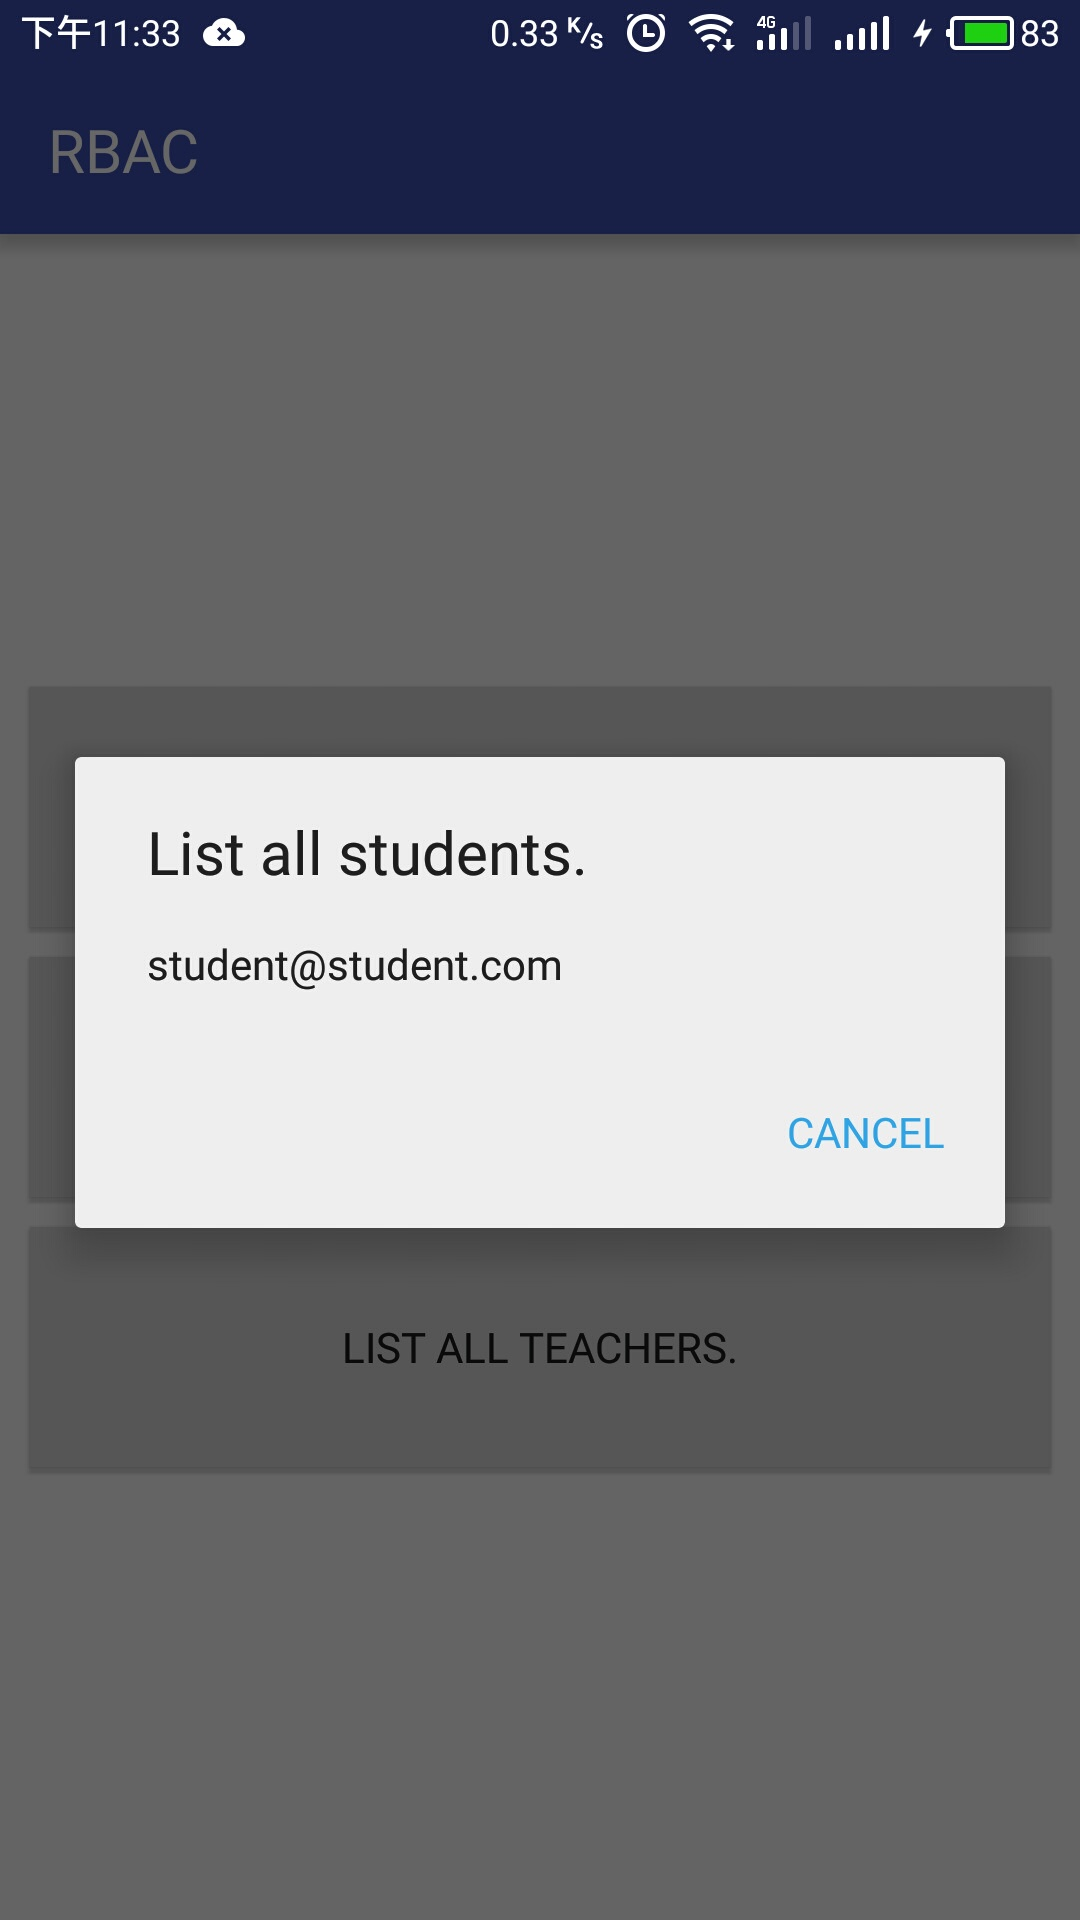
\includegraphics[height=0.39\textheight]{snapshot/17}
					\caption{管理员查看用户}
					\label{fig:17}
				\end{figure}
			
				\item 管理员查看教师用户:
				\begin{figure}[H]
					\centering
					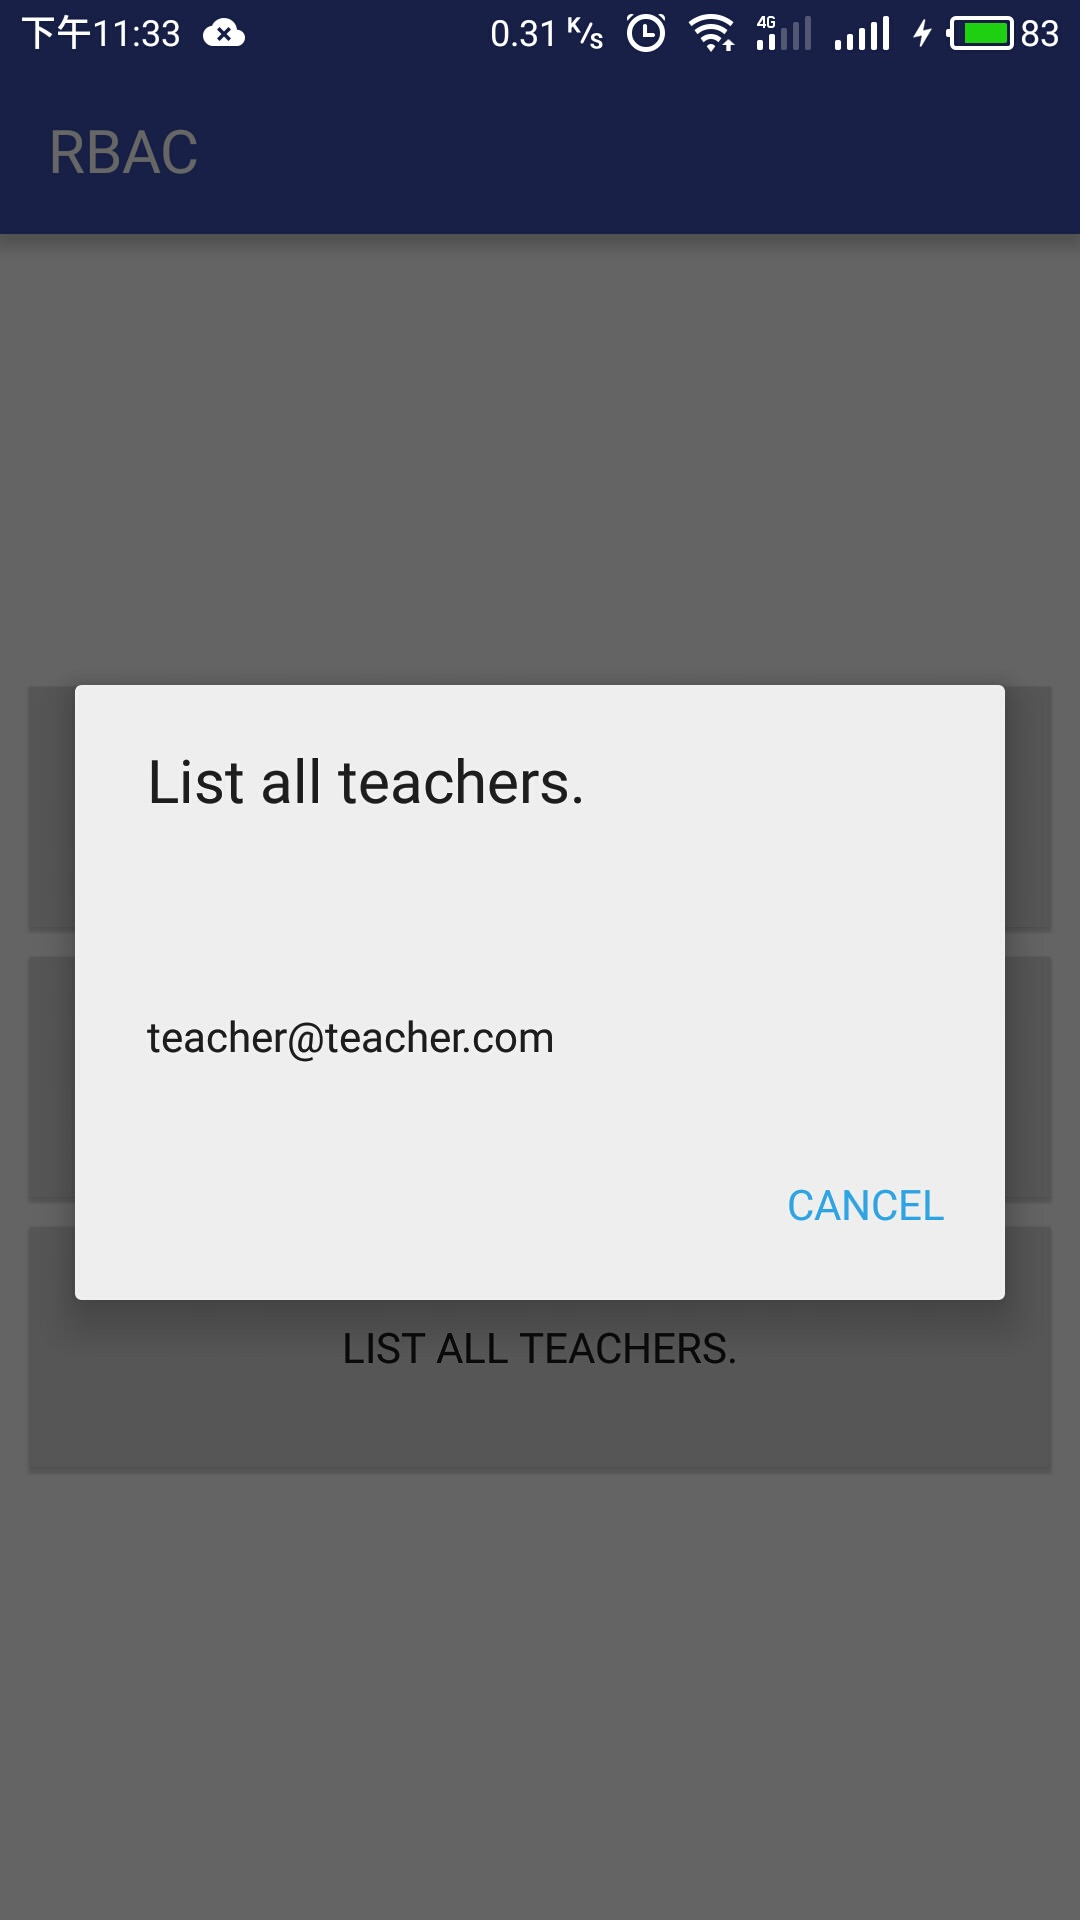
\includegraphics[height=0.39\textheight]{snapshot/18}
					\caption{管理员查看用户}
					\label{fig:18}
				\end{figure}
			\end{enumerate}
		
		\item
		整个Demo的功能基本就是这样,在角色权限的控制方面,我定义了这总共5个按钮的权限矩阵,使得每一种角色都对应这个矩阵的一行,以达到权限控制的目的。
		\item
		每一个用户的信息都由特定格式存储:[Email]:[Role];如系统初始化时就存在一个管理员账户为:hello@hello.com:admin。
		\item
		所以对于角色权限的修改是十分简单的,只需要改变矩阵中某个元素的值即可。
		
		\item 看一下关键源码:
		\begin{enumerate}
			\item 第一个Activity的Oncreate函数:
					\begin{lstlisting}[language=Java]
@Override
protected void onCreate(Bundle savedInstanceState) {

super.onCreate(savedInstanceState);
setContentView(R.layout.activity_login);

// Set up the login form.
mEmailView = (AutoCompleteTextView)
findViewById(R.id.email);
populateAutoComplete();

Button signIn = (Button) 
findViewById(R.id.email_sign_in_button);
Button registerButton = (Button) 
findViewById(R.id.register);
final RadioButton radioButtonTeacher 
= (RadioButton) 
findViewById(R.id.radioButtonTeacher);
RadioButton radioButtonStudent 
= (RadioButton) 
findViewById(R.id.radioButtonStudent);

signIn.setOnClickListener(new OnClickListener() {
@Override
public void onClick(View view) {
attemptLogin();
}
});

registerButton.setOnClickListener(new OnClickListener() {
@Override
public void onClick(View v) {
String newEmail = mEmailView.getText().toString();
for (String username : usernamePassword) {
String[] pieces = username.split(":");
if (pieces[0].equals(newEmail)) {
Toast.makeText(LoginActivity.this, 
"This email has been used.", Toast.LENGTH_SHORT)
.show();
return;
}
}
if (radioButtonTeacher.isChecked()) {
usernamePassword.add(newEmail + ":teacher");
} else {
usernamePassword.add(newEmail + ":student");
}
}
});

mLoginFormView = findViewById(R.id.login_form);
mProgressView = findViewById(R.id.login_progress);
}
			\end{lstlisting}
			第一个Activity主要处理了一些登录注册的逻辑,注册则先判断Email是否已经被注册过,登录的话则使用另一个继承自AsyncTask<Void, Void, Boolean>的内部类UserLoginTask来发送登录的异步请求(毕竟实际情况中可能会遭遇网络延时等情况);若登录成功,则把role放到Bundle中发送到第二个Activity。
			
			\item 第二个Activity的Oncreate函数:
			\begin{lstlisting}[language=Java]
@Override
public void onCreate(Bundle savedInstanceState) {
super.onCreate(savedInstanceState);
setContentView(R.layout.new_layout);

username = LoginActivity.getUsernamePassword();

Button[] buttons = {
(Button) findViewById(R.id.Imastudent),
(Button) findViewById(R.id.Imateacher),
(Button) findViewById(R.id.Imanadmin),
(Button) findViewById(R.id.Listallstudents),
(Button) findViewById(R.id.Listallteachers)};

buttons[0].setOnClickListener(
new View.OnClickListener() {
@Override
public void onClick(View v) {
new StudentDialog()
	.show(getFragmentManager(), "");
}
});

buttons[1].setOnClickListener(
new View.OnClickListener() {
@Override
public void onClick(View v) {
new TeacherDialog()
	.show(getFragmentManager(), "");
}
});

buttons[2].setOnClickListener(
new View.OnClickListener() {
@Override
public void onClick(View v) {
new AdminDialog()
	.show(getFragmentManager(), "");
}
});

buttons[3].setOnClickListener(
new View.OnClickListener() {
@Override
public void onClick(View v) {
List<String> studentList
	= new ArrayList<String>();
for (String name : username) {
String[] pieces = name.split(":");
if (pieces[1].equals("student")) {
studentList.add(pieces[0]);
}
}
String[] studentStr
	= new String[studentList.size()];
for (int i = 0; i < studentStr.length; ++i) {
studentStr[i] = studentList.get(i);
}
ListStudentDialog listStudentDialog 
	= new ListStudentDialog(studentStr);
listStudentDialog
	.show(getFragmentManager(), "");
}
});

buttons[4].setOnClickListener(
new View.OnClickListener() {
@Override
public void onClick(View v) {
List<String> studentList 
	= new ArrayList<String>();
for (String name : username) {
String[] pieces = name.split(":");
if (pieces[1].equals("teacher")) {
studentList.add(pieces[0]);
}
}

String[] teacherStr 
	= new String[studentList.size()];
for (int i = 0; i < teacherStr.length; ++i) {
teacherStr[i] = studentList.get(i);
}
ListTeacherDialog listTeacherDialog 
	= new ListTeacherDialog(teacherStr);
listTeacherDialog
	.show(getFragmentManager(), "");
}
});
String role 
	= getIntent().getStringExtra("role");
int[] permission = null;
switch (role) {
case "admin":
permission = adminPermission;
break;
case "teacher":
permission = teacherPermission;
break;
case "student":
permission = studentPermission;
break;
}

for (int i = 0; i < permission.length; ++i) {
if (permission[i] == 0) {
buttons[i].setVisibility(View.GONE);
}
}
}
			\end{lstlisting}
			
			\newpage
			可以看到所有的角色都跳转到一个有着5个Button的页面,这5个Button分别行使各自不同的逻辑;通过权限的矩阵进行Button可见性和可用性的控制,从而达到RBAC。
		\end{enumerate}

		\end{itemize}
	\end{enumerate}
\end{itemize}
